               %% bare_jrnl.tex
%% V1.4b
%% 2015/08/26
%% by Michael Shell
%% see http://www.michaelshell.org/
%% for current contact information.
%%
%% This is a skeleton file demonstrating the use of IEEEtran.cls
%% (requires IEEEtran.cls version 1.8b or later) with an IEEE
%% journal paper.
%%
%% Support sites:
%% http://www.michaelshell.org/tex/ieeetran/
%% http://www.ctan.org/pkg/ieeetran
%% and
%% http://www.ieee.org/

%%*************************************************************************
%% Legal Notice:
%% This code is offered as-is without any warranty either expressed or
%% implied; without even the implied warranty of MERCHANTABILITY or
%% FITNESS FOR A PARTICULAR PURPOSE! 
%% User assumes all risk.
%% In no event shall the IEEE or any contributor to this code be liable for
%% any damages or losses, including, but not limited to, incidental,
%% consequential, or any other damages, resulting from the use or misuse
%% of any information contained here.
%%
%% All comments are the opinions of their respective authors and are not
%% necessarily endorsed by the IEEE.
%%
%% This work is distributed under the LaTeX Project Public License (LPPL)
%% ( http://www.latex-project.org/ ) version 1.3, and may be freely used,
%% distributed and modified. A copy of the LPPL, version 1.3, is included
%% in the base LaTeX documentation of all distributions of LaTeX released
%% 2003/12/01 or later.
%% Retain all contribution notices and credits.
%% ** Modified files should be clearly indicated as such, including  **
%% ** renaming them and changing author support contact information. **
%%*************************************************************************


% *** Authors should verify (and, if needed, correct) their LaTeX system  ***
% *** with the testflow diagnostic prior to trusting their LaTeX platform ***
% *** with production work. The IEEE's font choices and paper sizes can   ***
% *** trigger bugs that do not appear when using other class files.       ***                          ***
% The testflow support page is at:
% http://www.michaelshell.org/tex/testflow/


% Please refer to your journal's instructions for other
% options that should be set.
\documentclass[journal,onecolumn, 11pt]{IEEEtran}
%
% If IEEEtran.cls has not been installed into the LaTeX system files,
% manually specify the path to it like:
% \documentclass[journal]{../sty/IEEEtran}





% Some very useful LaTeX packages include:
% (uncomment the ones you want to load)


% *** MISC UTILITY PACKAGES ***
%
%\usepackage{ifpdf}
% Heiko Oberdiek's ifpdf.sty is very useful if you need conditional
% compilation based on whether the output is pdf or dvi.
% usage:
% \ifpdf
%   % pdf code
% \else
%   % dvi code
% \fi
% The latest version of ifpdf.sty can be obtained from:
% http://www.ctan.org/pkg/ifpdf
% Also, note that IEEEtran.cls V1.7 and later provides a builtin
% \ifCLASSINFOpdf conditional that works the same way.
% When switching from latex to pdflatex and vice-versa, the compiler may
% have to be run twice to clear warning/error messages.






% *** CITATION PACKAGES ***
%
%\usepackage{cite}
% cite.sty was written by Donald Arseneau
% V1.6 and later of IEEEtran pre-defines the format of the cite.sty package
% \cite{} output to follow that of the IEEE. Loading the cite package will
% result in citation numbers being automatically sorted and properly
% "compressed/ranged". e.g., [1], [9], [2], [7], [5], [6] without using
% cite.sty will become [1], [2], [5]--[7], [9] using cite.sty. cite.sty's
% \cite will automatically add leading space, if needed. Use cite.sty's
% noadjust option (cite.sty V3.8 and later) if you want to turn this off
% such as if a citation ever needs to be enclosed in parenthesis.
% cite.sty is already installed on most LaTeX systems. Be sure and use
% version 5.0 (2009-03-20) and later if using hyperref.sty.
% The latest version can be obtained at:
% http://www.ctan.org/pkg/cite
% The documentation is contained in the cite.sty file itself.






% *** GRAPHICS RELATED PACKAGES ***
%
\ifCLASSINFOpdf
  % \usepackage[pdftex]{graphicx}
  % declare the path(s) where your graphic files are
  % \graphicspath{{../pdf/}{../jpeg/}}
  % and their extensions so you won't have to specify these with
  % every instance of \includegraphics
  % \DeclareGraphicsExtensions{.pdf,.jpeg,.png}
\else
  % or other class option (dvipsone, dvipdf, if not using dvips). graphicx
  % will default to the driver specified in the system graphics.cfg if no
  % driver is specified.
  % \usepackage[dvips]{graphicx}
  % declare the path(s) where your graphic files are
  % \graphicspath{{../eps/}}
  % and their extensions so you won't have to specify these with
  % every instance of \includegraphics
  % \DeclareGraphicsExtensions{.eps}
\fi
% graphicx was written by David Carlisle and Sebastian Rahtz. It is
% required if you want graphics, photos, etc. graphicx.sty is already
% installed on most LaTeX systems. The latest version and documentation
% can be obtained at: 
% http://www.ctan.org/pkg/graphicx
% Another good source of documentation is "Using Imported Graphics in
% LaTeX2e" by Keith Reckdahl which can be found at:
% http://www.ctan.org/pkg/epslatex
%
% latex, and pdflatex in dvi mode, support graphics in encapsulated
% postscript (.eps) format. pdflatex in pdf mode supports graphics
% in .pdf, .jpeg, .png and .mps (metapost) formats. Users should ensure
% that all non-photo figures use a vector format (.eps, .pdf, .mps) and
% not a bitmapped formats (.jpeg, .png). The IEEE frowns on bitmapped formats
% which can result in "jaggedy"/blurry rendering of lines and letters as
% well as large increases in file sizes.
%
% You can find documentation about the pdfTeX application at:
% http://www.tug.org/applications/pdftex





% *** MATH PACKAGES ***
%
%\usepackage{amsmath}
% A popular package from the American Mathematical Society that provides
% many useful and powerful commands for dealing with mathematics.
%
% Note that the amsmath package sets \interdisplaylinepenalty to 10000
% thus preventing page breaks from occurring within multiline equations. Use:
%\interdisplaylinepenalty=2500
% after loading amsmath to restore such page breaks as IEEEtran.cls normally
% does. amsmath.sty is already installed on most LaTeX systems. The latest
% version and documentation can be obtained at:
% http://www.ctan.org/pkg/amsmath





% *** SPECIALIZED LIST PACKAGES ***
%
%\usepackage{algorithmic}
% algorithmic.sty was written by Peter Williams and Rogerio Brito.
% This package provides an algorithmic environment fo describing algorithms.
% You can use the algorithmic environment in-text or within a figure
% environment to provide for a floating algorithm. Do NOT use the algorithm
% floating environment provided by algorithm.sty (by the same authors) or
% algorithm2e.sty (by Christophe Fiorio) as the IEEE does not use dedicated
% algorithm float types and packages that provide these will not provide
% correct IEEE style captions. The latest version and documentation of
% algorithmic.sty can be obtained at:
% http://www.ctan.org/pkg/algorithms
% Also of interest may be the (relatively newer and more customizable)
% algorithmicx.sty package by Szasz Janos:
% http://www.ctan.org/pkg/algorithmicx




% *** ALIGNMENT PACKAGES ***
%
%\usepackage{array}
% Frank Mittelbach's and David Carlisle's array.sty patches and improves
% the standard LaTeX2e array and tabular environments to provide better
% appearance and additional user controls. As the default LaTeX2e table
% generation code is lacking to the point of almost being broken with
% respect to the quality of the end results, all users are strongly
% advised to use an enhanced (at the very least that provided by array.sty)
% set of table tools. array.sty is already installed on most systems. The
% latest version and documentation can be obtained at:
% http://www.ctan.org/pkg/array


% IEEEtran contains the IEEEeqnarray family of commands that can be used to
% generate multiline equations as well as matrices, tables, etc., of high
% quality.




% *** SUBFIGURE PACKAGES ***
%\ifCLASSOPTIONcompsoc
%  \usepackage[caption=false,font=normalsize,labelfont=sf,textfont=sf]{subfig}
%\else
%  \usepackage[caption=false,font=footnotesize]{subfig}
%\fi
% subfig.sty, written by Steven Douglas Cochran, is the modern replacement
% for subfigure.sty, the latter of which is no longer maintained and is
% incompatible with some LaTeX packages including fixltx2e. However,
% subfig.sty requires and automatically loads Axel Sommerfeldt's caption.sty
% which will override IEEEtran.cls' handling of captions and this will result
% in non-IEEE style figure/table captions. To prevent this problem, be sure
% and invoke subfig.sty's "caption=false" package option (available since
% subfig.sty version 1.3, 2005/06/28) as this is will preserve IEEEtran.cls
% handling of captions.
% Note that the Computer Society format requires a larger sans serif font
% than the serif footnote size font used in traditional IEEE formatting
% and thus the need to invoke different subfig.sty package options depending
% on whether compsoc mode has been enabled.
%
% The latest version and documentation of subfig.sty can be obtained at:
% http://www.ctan.org/pkg/subfig




% *** FLOAT PACKAGES ***
%
%\usepackage{fixltx2e}
% fixltx2e, the successor to the earlier fix2col.sty, was written by
% Frank Mittelbach and David Carlisle. This package corrects a few problems
% in the LaTeX2e kernel, the most notable of which is that in current
% LaTeX2e releases, the ordering of single and double column floats is not
% guaranteed to be preserved. Thus, an unpatched LaTeX2e can allow a
% single column figure to be placed prior to an earlier double column
% figure.
% Be aware that LaTeX2e kernels dated 2015 and later have fixltx2e.sty's
% corrections already built into the system in which case a warning will
% be issued if an attempt is made to load fixltx2e.sty as it is no longer
% needed.
% The latest version and documentation can be found at:
% http://www.ctan.org/pkg/fixltx2e


%\usepackage{stfloats}
% stfloats.sty was written by Sigitas Tolusis. This package gives LaTeX2e
% the ability to do double column floats at the bottom of the page as well
% as the top. (e.g., "\begin{figure*}[!b]" is not normally possible in
% LaTeX2e). It also provides a command:
%\fnbelowfloat
% to enable the placement of footnotes below bottom floats (the standard
% LaTeX2e kernel puts them above bottom floats). This is an invasive package
% which rewrites many portions of the LaTeX2e float routines. It may not work
% with other packages that modify the LaTeX2e float routines. The latest
% version and documentation can be obtained at:
% http://www.ctan.org/pkg/stfloats
% Do not use the stfloats baselinefloat ability as the IEEE does not allow
% \baselineskip to stretch. Authors submitting work to the IEEE should note
% that the IEEE rarely uses double column equations and that authors should try
% to avoid such use. Do not be tempted to use the cuted.sty or midfloat.sty
% packages (also by Sigitas Tolusis) as the IEEE does not format its papers in
% such ways.
% Do not attempt to use stfloats with fixltx2e as they are incompatible.
% Instead, use Morten Hogholm'a dblfloatfix which combines the features
% of both fixltx2e and stfloats:
%
% \usepackage{dblfloatfix}
% The latest version can be found at:
% http://www.ctan.org/pkg/dblfloatfix




%\ifCLASSOPTIONcaptionsoff
%  \usepackage[nomarkers]{endfloat}
% \let\MYoriglatexcaption\caption
% \renewcommand{\caption}[2][\relax]{\MYoriglatexcaption[#2]{#2}}
%\fi
% endfloat.sty was written by James Darrell McCauley, Jeff Goldberg and 
% Axel Sommerfeldt. This package may be useful when used in conjunction with 
% IEEEtran.cls'  captionsoff option. Some IEEE journals/societies require that
% submissions have lists of figures/tables at the end of the paper and that
% figures/tables without any captions are placed on a page by themselves at
% the end of the document. If needed, the draftcls IEEEtran class option or
% \CLASSINPUTbaselinestretch interface can be used to increase the line
% spacing as well. Be sure and use the nomarkers option of endfloat to
% prevent endfloat from "marking" where the figures would have been placed
% in the text. The two hack lines of code above are a slight modification of
% that suggested by in the endfloat docs (section 8.4.1) to ensure that
% the full captions always appear in the list of figures/tables - even if
% the user used the short optional argument of \caption[]{}.
% IEEE papers do not typically make use of \caption[]'s optional argument,
% so this should not be an issue. A similar trick can be used to disable
% captions of packages such as subfig.sty that lack options to turn off
% the subcaptions:
% For subfig.sty:
% \let\MYorigsubfloat\subfloat
% \renewcommand{\subfloat}[2][\relax]{\MYorigsubfloat[]{#2}}
% However, the above trick will not work if both optional arguments of
% the \subfloat command are used. Furthermore, there needs to be a
% description of each subfigure *somewhere* and endfloat does not add
% subfigure captions to its list of figures. Thus, the best approach is to
% avoid the use of subfigure captions (many IEEE journals avoid them anyway)
% and instead reference/explain all the subfigures within the main caption.
% The latest version of endfloat.sty and its documentation can obtained at:
% http://www.ctan.org/pkg/endfloat
%
% The IEEEtran \ifCLASSOPTIONcaptionsoff conditional can also be used
% later in the document, say, to conditionally put the References on a 
% page by themselves.




% *** PDF, URL AND HYPERLINK PACKAGES ***
%
%\usepackage{url}
% url.sty was written by Donald Arseneau. It provides better support for
% handling and breaking URLs. url.sty is already installed on most LaTeX
% systems. The latest version and documentation can be obtained at:
% http://www.ctan.org/pkg/url
% Basically, \url{my_url_here}.




% *** Do not adjust lengths that control margins, column widths, etc. ***
% *** Do not use packages that alter fonts (such as pslatex).         ***
% There should be no need to do such things with IEEEtran.cls V1.6 and later.
% (Unless specifically asked to do so by the journal or conference you plan
% to submit to, of course. )


% \documentclass[12pt]{article}
% \usepackage[utf8]{inputenc}
% \usepackage{geometry}
% \geometry{a4paper, margin=1in}
\usepackage{amsmath}
\usepackage{graphicx}
\usepackage{hyperref}
\usepackage{array}
\usepackage{times}
\usepackage{float}
\setlength{\parindent}{2em}
% \addto\captionsvietnamese{\renewcommand{\refname}{References}}
% \addto\captionsvietnamese{\renewcommand{\tablename}{Table}}
\usepackage{ragged2e}
\usepackage{subfigure}   
\usepackage{multirow}
\usepackage{caption}

% correct bad hyphenation here
\hyphenation{op-tical net-works semi-conduc-tor}


\begin{document}
%
% paper title
% Titles are generally capitalized except for words such as a, an, and, as,
% at, but, by, for, in, nor, of, on, or, the, to and up, which are usually
% not capitalized unless they are the first or last word of the title.
% Linebreaks \\ can be used within to get better formatting as desired.
% Do not put math or special symbols in the title.
\title{Comparative and Combined Study of Deep Learning Techniques for Gym Exercise Classification}
% \title{Combining Sequential and Graph-Based Temporal Models for Gym Exercise Recognition}
%
%
% author names and IEEE memberships
% note positions of commas and nonbreaking spaces ( ~ ) LaTeX will not break
% a structure at a ~ so this keeps an author's name from being broken across
% two lines.
% use \thanks{} to gain access to the first footnote area
% a separate \thanks must be used for each paragraph as LaTeX2e's \thanks
% was not built to handle multiple paragraphs
%

\author{Xuan-Cuong Nguyen,%~\IEEEmembership{,~IEEE,}
        ~Nhat-Quang Truong,%~\IEEEmembership{Fellow,~OSA,}
        

\texttt{cuongnxde180528@fpt.edu.vn} \\
FPT University, Da Nang
\thanks{FPT \copyright2025 ResFes}
% of Electrical and Computer Engineering, Georgia Institute of Technology, Atlanta,
% GA, 30332 USA e-mail: (see http://www.michaelshell.org/contact.html).}% <-this % stops a space
% \thanks{J. Doe and J. Doe are with Anonymous University.}% <-this % stops a space
% \thanks{Manuscript received April 19, 2005; revised August 26, 2015.}
}

% note the % following the last \IEEEmembership and also \thanks - 
% these prevent an unwanted space from occurring between the last author name
% and the end of the author line. i.e., if you had this:
% 
% \author{....lastname \thanks{...} \thanks{...} }
%                     ^------------^------------^----Do not want these spaces!
%
% a space would be appended to the last name and could cause every name on that
% line to be shifted left slightly. This is one of those "LaTeX things". For
% instance, "\textbf{A} \textbf{B}" will typeset as "A B" not "AB". To get
% "AB" then you have to do: "\textbf{A}\textbf{B}"
% \thanks is no different in this regard, so shield the last } of each \thanks
% that ends a line with a % and do not let a space in before the next \thanks.
% Spaces after \IEEEmembership other than the last one are OK (and needed) as
% you are supposed to have spaces between the names. For what it is worth,
% this is a minor point as most people would not even notice if the said evil
% space somehow managed to creep in.



% The paper headers
% \markboth{Journal of \LaTeX\ Class Files,~Vol.~14, No.~8, August~2015}%
% {Shell \MakeLowercase{\textit{et al.}}: Bare Demo of IEEEtran.cls for IEEE Journals}
% The only time the second header will appear is for the odd numbered pages
% after the title page when using the twoside option.
% 
% *** Note that you probably will NOT want to include the author's ***
% *** name in the headers of peer review papers.                   ***
% You can use \ifCLASSOPTIONpeerreview for conditional compilation here if
% you desire.




% If you want to put a publisher's ID mark on the page you can do it like
% this:
%\IEEEpubid{0000--0000/00\$00.00~\copyright~2015 IEEE}
% Remember, if you use this you must call \IEEEpubidadjcol in the second
% column for its text to clear the IEEEpubid mark.



% use for special paper notices
%\IEEEspecialpapernotice{(Invited Paper)}




% make the title area
\maketitle

% As a general rule, do not put math, special symbols or citations
% in the abstract or keywords.
\begin{abstract}
% This paper proposes a three-branch pipeline for classifying 22 gym exercises. 
% Videos from a public Workout/Exercise dataset, YouTube and author recordings are manually trimmed into clean segments and sampled into overlapping clips of 32 frames with a 16-frame overlap (padding the last frame when necessary). 
% In the pose branch, MediaPipe extracts 13 key 2D landmarks and computes joint-angle features, which are modeled by LSTM, Bi-LSTM and Transformer encoders. 
% The CNN branch fine-tunes InceptionV3 to obtain multi-scale feature maps (Blocks 2, 5, 10), each processed by LSTM, Bi-LSTM or Transformer modules. 
% The 3D branch inputs raw clips into Swin3D, where all but the last Transformer stage, layer-norm parameters and classification head are frozen; only these final layers are fine-tuned (Tiny pre-trained on Kinetics-400; Base pre-trained on ImageNet-22K + Kinetics-400). 
% Final predictions are obtained by late-fusion of the softmax outputs from the best pose Transformer and the Swin3D-Base model. 
% Experiments on 885 clips demonstrate that our ensemble reaches 79.46\% accuracy on the held-out test set, validating the complementary strengths of skeletal and full-frame representations.
%%%%%%%%%%%%%%%%%%%%%%%%%%%%%%%%
% This paper proposes a method to classify gym exercises using computer vision.
% In the proposed method, videos are preprocessed before landmark features of their frames are extracted using MediaPie.
% Extracted landmark features are then augmented to increase the number of instances in training set which are used to feed to transformer model.
% Augmentation stage after landmark feature extraction can enhance training deep learning models while reducing  processing time compared to that of the augmentation of original videos.
% Experiments on self-collected dataset are carried out to confirm effectiveness of the proposed method.
% Experimental results on 885 clips of 22 different types of gym exercises show that the proposed method can improve overall accuracy 4\% in comparison with the existing method.
%%%%%%%%%%%%%%%%%%%%%%%%%%%%%%%%%%
% Raw gym videos are first trimmed into clean segments and sampled into fixed‐length clips for downstream processing. Our three‐branch framework then extracts complementary representations: (1) a pose stream in which MediaPipe detects 13 key 2D landmarks per frame—re-centered on the nose and converted into relative joint‐angle features—then modeled by a lightweight Transformer encoder; (2) a CNN stream that leverages multi‐scale activation maps (288-D from Block 2, 768-D from Block 5, and 2048-D from Block 10) extracted by InceptionV3 and processed through spatio‐temporal modules; and (3) a 3D video stream where non-overlapping 32-frame clips are input directly into a Swin3D transformer, fine-tuning only its final attention stages, normalization layers, and classification head. 
% Experimental results on a self-collected dataset of 887 clips spanning 22 gym exercises show that the Swin3D model achieves the highest accuracy of 69.8\%, outperforming both the pose‐only and CNN‐only streams. 
% These results underscore the effectiveness of hierarchical spatio-temporal attention for robust, real-time exercise recognition.

% Raw gym videos are first trimmed into clean segments and sampled into fixed‐length clips for downstream processing. Our two-branch framework then extracts complementary representations: (1) a pose stream in which MediaPipe detects 13 key 2D landmarks per frame—re-centered on the nose and converted into relative joint-angle features—then modeled by a lightweight Transformer encoder; and (2) a CNN stream that leverages multi-scale activation maps (288-D from Block 2, 768-D from Block 5, and 2048-D from Block 10) extracted by InceptionV3 and processed through spatio-temporal modules.
% Experimental results on a self-collected dataset of 887 clips spanning 22 gym exercises demonstrate that combining both pose-based and appearance-based streams significantly improves classification performance over either one alone.
% These findings highlight the benefit of fusing skeletal motion and visual semantics for accurate, real-time exercise recognition.
Raw gym videos are first manually trimmed into clean segments and sampled into fixed‐length clips for downstream processing. We propose a dual‐branch framework that captures both skeletal and graph‐based representations: a pose stream in which MediaPipe detects 33 key 3D landmarks per frame—each re‐centered on the nose and converted into relative coordinates and joint angles computed via triplet permutations—and modeled with a lightweight Transformer encoder; and a graph stream that constructs a spatio‐temporal joint graph from the same landmarks and processes it through an ST‐GCN to directly learn dynamic relationships among connected joints. We evaluate our approach on a self‐collected dataset of 1 026 clean clips covering 22 common gym exercises. Experimental results demonstrate that fusing landmark‐based features with explicit graph‐convolutional modeling yields substantially higher classification accuracy than either branch alone, underscoring the importance of combining relative skeletal cues and structured joint dynamics for accurate, real‐time exercise recognition.

\end{abstract}

% Note that keywords are not normally used for peerreview papers.
\begin{IEEEkeywords}
Gym exercise classification, pose estimation, MediaPipe, ST-GCN, LSTM, Transformer, feature engineering, temporal modeling, human action recognition.
\end{IEEEkeywords}






% For peer review papers, you can put extra information on the cover
% page as needed:
% \ifCLASSOPTIONpeerreview
% \begin{center} \bfseries EDICS Category: 3-BBND \end{center}
% \fi
%
% For peerreview papers, this IEEEtran command inserts a page break and
% creates the second title. It will be ignored for other modes.
\IEEEpeerreviewmaketitle



\section{Introduction}
% The very first letter is a 2 line initial drop letter followed
% by the rest of the first word in caps.
% 
% form to use if the first word consists of a single letter:
% \IEEEPARstart{A}{demo} file is ....
% 
% form to use if you need the single drop letter followed by
% normal text (unknown if ever used by the IEEE):
% \IEEEPARstart{A}{}demo file is ....
% 
% Some journals put the first two words in caps:
% \IEEEPARstart{T}{his demo} file is ....
% 
% Here we have the typical use of a "T" for an initial drop letter
% and "HIS" in caps to complete the first word.
% \IEEEPARstart{T}{his} demo file is intended to serve as a ``starter file''
% for IEEE journal papers produced under \LaTeX\ using
% IEEEtran.cls version 1.8b and later.
% % You must have at least 2 lines in the paragraph with the drop letter
% % (should never be an issue)
% I wish you the best of success.

% \hfill %mds
 
% \hfill %August 26, 2015

% \subsection{Research objectives}
% The goal of this work is to develop a real-time exercise classification system using pose estimation and video-based features. We evaluate multiple deep learning architectures—LSTM, Bi-LSTM, Transformer, InceptionV3 and Swin3D (both Tiny and Base variants)—to automatically recognize gym movements. By combining invariant joint-angle features with raw landmark coordinates, the system is designed to be robust to variations in body shape, camera viewpoint and lighting. We benchmark our approaches against existing methods on the dataset’s held-out test set to ensure fair comparison. Future work will extend beyond simple classification toward assessing exercise form quality rather than counting repetitions.

% \subsection{The necessity of the research}
% Maintaining regular exercise is vital for both physical and mental well-being, yet many people struggle with improper technique, difficulty tracking progress, and lack of personalized feedback, resulting in poor adherence. Manual counting or relying on a personal trainer can be inconvenient or costly. Advances in pose estimation and deep learning promise automated exercise recognition, but existing solutions that depend on raw coordinates or frame-level classification often fail when faced with different body types, camera angles or lighting conditions. A robust, real-time system combining pose-based features with sequence models is therefore needed to provide accurate and generalizable exercise classification.

% When life quality improves day by day, gym becomes an important sport as it can help people to enhance both mental and physical health.
% Because of its benefits, there are many people doing gym exercises in fitness centers or at home.
% In the scenario of lack of time, people would prefer to select the second option rather than the first.
% However, many people often do not know how to do gym exercises correctly.
% It is important because incorrect pose when doing gym exercises could cause a negative effect or injuries on individual body.
% Therefore, for individuals who do gym exercises at home, it is necessary to have a virtual personal trainer to observe and recommend them to avoid doing an abnormal pose.
% In order to realize this type of the system, the first step is to recognize the type of gym exercise that individual is doing.
% Fortunately, the development of machine learning and deep learning algorithms allows the system to which they are integrated to realize classification task with high accuracy in both images and videos.
% Specially, they can recognize the words in sign language using images or videos \cite{Mahyoub2024} or estimating human pose in sorts training \cite{Xi2024}.

% In the existing studies, the deep learning models were trained and evaluated on a few classes of gym exercises which would reduce the generalizability of the models, leading to the difficulty in realizing virtual personal trainer. 
% In this study, a deep learning based method is proposed to realize the classification task for different types of gym exercises.
% In comparison with the existing studies, deep learning model is trained and evaluated on 885 clips of 22 different types of gym exercises which are collected from different public data.
% Firstly, MediaPie is used to extract landmark features from the frames of the videos.
% Then, these features are augmented to enhance the training phase for deep learning models.
% In compared to augmenting original videos, this method has a lower complexity while still improving  overall accuracy.


As general living standards rise, more individuals turn to gym workouts to bolster both physical fitness and mental well–being. Yet without expert supervision, home exercisers often adopt incorrect form, risking injury or suboptimal results. A virtual personal trainer must first recognize which exercise is being performed; only then can it deliver timely feedback and correction. Recent advances in deep learning—especially video transformers—make it possible to tackle this recognition task with high accuracy directly from raw footage.

% In this study, we introduce a three-branch framework for gym exercise classification. The pose branch leverages MediaPipe to extract 13 key 2D landmarks per frame, re-centered on the nose and converted into relative joint-angle features; these sequences are modeled by a compact Transformer encoder. The CNN branch employs an InceptionV3 backbone to harvest multi-scale activation maps (288-dim from Block 2, 768-dim from Block 5, and 2048-dim from Block 10), which are then processed by spatio-temporal modules (LSTM, Bi-LSTM, or Transformer). Finally, the Swin3D branch ingests non-overlapping 32-frame clips directly into a 3D Transformer architecture, fine-tuning only its final transformer stage, normalization layers, and classification head. Experiments on 887 clips spanning 22 gym exercises demonstrate that the Swin3D branch alone achieves 69.8\% test accuracy, substantially outperforming both the pose-only and CNN-only streams.

% In this study, we introduce a two-branch framework for gym exercise classification. The pose branch leverages MediaPipe to extract 13 key 2D landmarks per frame, re-centered on the nose and converted into relative joint-angle features; these sequences are modeled by a compact Transformer encoder. The CNN branch employs an InceptionV3 backbone to harvest multi-scale activation maps (288-dim from Block 2, 768-dim from Block 5, and 2048-dim from Block 10), which are then processed by spatio-temporal modules such as LSTM, Bi-LSTM, or Transformer layers.
% Experiments on 887 clips spanning 22 gym exercises show that the combination of pose and CNN streams yields competitive classification performance, with each stream capturing complementary aspects of body movement and visual context.

In this study, we introduce a two-branch framework for gym exercise classification. The pose branch leverages MediaPipe to extract 33 key 3D landmarks per frame—each re-centered on the nose and converted into relative coordinates and joint angles computed via triplet permutations—and models these feature sequences with a compact Transformer encoder. The graph branch constructs a spatio-temporal joint graph from the same landmarks and processes it through an ST-GCN to directly capture dynamic relationships between body joints. Experiments on a self-collected dataset of 1 026 clean clips spanning 22 gym exercises demonstrate that fusing landmark-based and graph-based representations significantly outperforms either branch alone, highlighting the benefit of combining relative skeletal features with explicit joint-graph modeling for accurate, real-time exercise recognition.


% needed in second column of first page if using \IEEEpubid
%\IEEEpubidadjcol

% \subsubsection{Subsubsection Heading Here}
% Subsubsection text here.




% An example of a floating figure using the graphicx package.
% Note that \label must occur AFTER (or within) \caption.
% For figures, \caption should occur after the \includegraphics.
% Note that IEEEtran v1.7 and later has special internal code that
% is designed to preserve the operation of \label within \caption
% even when the captionsoff option is in effect. However, because
% of issues like this, it may be the safest practice to put all your
% \label just after \caption rather than within \caption{}.
%
% Reminder: the "draftcls" or "draftclsnofoot", not "draft", class
% option should be used if it is desired that the figures are to be
% displayed while in draft mode.
%
%\begin{figure}[!t]
%\centering
%\includegraphics[width=2.5in]{myfigure}
% where an .eps filename suffix will be assumed under latex, 
% and a .pdf suffix will be assumed for pdflatex; or what has been declared
% via \DeclareGraphicsExtensions.
%\caption{Simulation results for the network.}
%\label{fig_sim}
%\end{figure}

% Note that the IEEE typically puts floats only at the top, even when this
% results in a large percentage of a column being occupied by floats.


% An example of a double column floating figure using two subfigures.
% (The subfig.sty package must be loaded for this to work.)
% The subfigure \label commands are set within each subfloat command,
% and the \label for the overall figure must come after \caption.
% \hfil is used as a separator to get equal spacing.
% Watch out that the combined width of all the subfigures on a 
% line do not exceed the text width or a line break will occur.
%
%\begin{figure*}[!t]
%\centering
%\subfloat[Case I]{\includegraphics[width=2.5in]{box}%
%\label{fig_first_case}}
%\hfil
%\subfloat[Case II]{\includegraphics[width=2.5in]{box}%
%\label{fig_second_case}}
%\caption{Simulation results for the network.}
%\label{fig_sim}
%\end{figure*}
%
% Note that often IEEE papers with subfigures do not employ subfigure
% captions (using the optional argument to \subfloat[]), but instead will
% reference/describe all of them (a), (b), etc., within the main caption.
% Be aware that for subfig.sty to generate the (a), (b), etc., subfigure
% labels, the optional argument to \subfloat must be present. If a
% subcaption is not desired, just leave its contents blank,
% e.g., \subfloat[].


% An example of a floating table. Note that, for IEEE style tables, the
% \caption command should come BEFORE the table and, given that table
% captions serve much like titles, are usually capitalized except for words
% such as a, an, and, as, at, but, by, for, in, nor, of, on, or, the, to
% and up, which are usually not capitalized unless they are the first or
% last word of the caption. Table text will default to \footnotesize as
% the IEEE normally uses this smaller font for tables.
% The \label must come after \caption as always.
%
%\begin{table}[!t]
%% increase table row spacing, adjust to taste
%\renewcommand{\arraystretch}{1.3}
% if using array.sty, it might be a good idea to tweak the value of
% \extrarowheight as needed to properly center the text within the cells
%\caption{An Example of a Table}
%\label{table_example}
%\centering
%% Some packages, such as MDW tools, offer better commands for making tables
%% than the plain LaTeX2e tabular which is used here.
%\begin{tabular}{|c||c|}
%\hline
%One & Two\\
%\hline
%Three & Four\\
%\hline
%\end{tabular}
%\end{table}


% Note that the IEEE does not put floats in the very first column
% - or typically anywhere on the first page for that matter. Also,
% in-text middle ("here") positioning is typically not used, but it
% is allowed and encouraged for Computer Society conferences (but
% not Computer Society journals). Most IEEE journals/conferences use
% top floats exclusively. 
% Note that, LaTeX2e, unlike IEEE journals/conferences, places
% footnotes above bottom floats. This can be corrected via the
% \fnbelowfloat command of the stfloats package.




\section{Related Work}

In 2015, Donahue et al. introduced a CNN-LSTM framework for action classification that integrated convolutional networks for spatial feature extraction with LSTM networks for temporal modeling. Their model, evaluated on datasets such as UCF101, reported a top-1 accuracy of approximately 82\% \cite{donahue2015}. Although this hybrid approach successfully captured both appearance and motion cues, it was hindered by high computational complexity and challenging training dynamics due to the integration of convolutional and recurrent components.

Building upon early CNN-LSTM methods, landmark-based LSTM approaches emerged around 2016. For instance, Li et al. (2016) proposed a method where skeletal keypoints are extracted via pose estimation and then fed into an LSTM network for action recognition. Evaluated on the NTU RGB+D dataset, their approach achieved roughly 86\% accuracy on the cross-subject protocol \cite{li2017}. This method benefits from a reduced computational load by focusing on essential body movements rather than full images; however, its performance is highly dependent on the quality of the underlying pose estimation, with inaccuracies in landmark extraction significantly affecting the final results.

In 2018, Yan et al. advanced the field with the introduction of the Spatial Temporal Graph Convolutional Network (ST-GCN), which models the human skeleton as a graph where keypoints serve as nodes and anatomical connections as edges. Tested on the NTU RGB+D dataset, ST-GCN obtained 81.5\% accuracy under the cross-subject setting and up to 88.3\% in the cross-view configuration \cite{yan2018}. The strength of ST-GCN lies in its simultaneous modeling of spatial configurations and temporal dynamics; nevertheless, its reliance on accurate skeleton extraction and predefined graph structures limits its robustness, especially in the presence of noisy or incomplete data.

More recently, the adoption of transformer-based architectures has led to further improvements in action classification. Arnab et al. (2021) extended the Vision Transformer (ViT) paradigm to the video domain with the ViViT model, which applies self-attention mechanisms over image patches to capture long-range dependencies across frames. Evaluated on the Kinetics-400 dataset, ViViT achieved a top-1 accuracy of approximately 77\% \cite{arnab2021}. Although transformer-based models excel at capturing global context, they require extensive training data and significant computational resources, which can be a critical limitation for practical deployment.

In 2024, Nguyen et al. extended landmark-based LSTM methods to exercise classification on a four-class dataset (barbell biceps curl, push-up, squat, shoulder press) by extracting 22 body keypoints and 12 joint-angle features per frame and feeding them into a bidirectional LSTM. Evaluated on 791 test windows, their BiLSTM model achieved near-perfect performance—overall accuracy of 0.99, with F1-scores of 0.99 for curl, 1.00 for push-up, 0.98 for squat, and 1.00 for shoulder press . They generated overlapping 30-frame windows from each video and then randomly shuffled all windows before splitting into train/validation/test sets at a 70\%–15\%–15\% ratio . While this approach yields impressive metrics, it permits windows from the same video to appear across different splits—introducing data leakage that inflates test performance—and relies on a fixed window length that may not generalize well to varying movement speeds or durations.  \cite{riccio2024}

Overall, these studies reflect a progressive evolution in action recognition. Early methods such as CNN-LSTM and landmark-based LSTM provide effective spatial-temporal integration, yet they face challenges related to computational cost and sensitivity to input quality, respectively. In contrast, ST-GCN leverages the structural information of the human skeleton but depends on high-quality pose data, while transformer-based approaches like ViViT offer superior global context modeling at the expense of increased data and computational requirements. These varied outcomes underscore the importance of developing robust systems that blend the complementary strengths of these techniques for efficient and accurate action classification.



\section{Dataset}


\begin{figure}[H]
    % \hspace*{-1.5cm} % <-- Đẩy ảnh qua bên trái
    \begin{center}
    \resizebox{0.9\textwidth}{!}{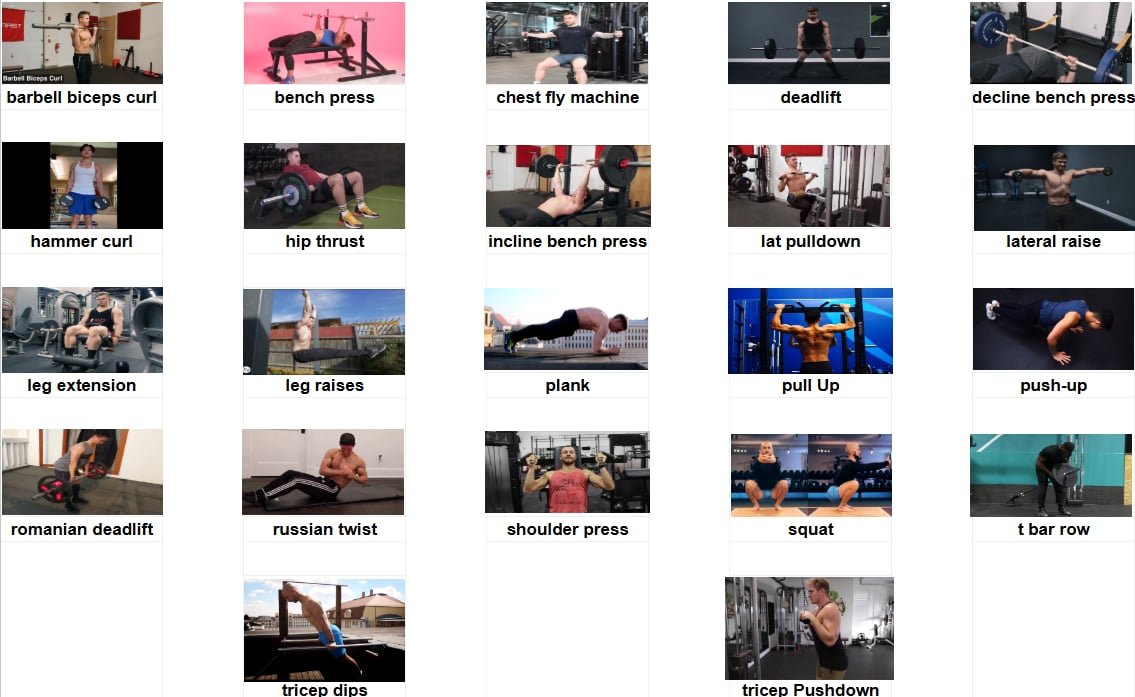
\includegraphics{Dataset.png}}
    \end{center}
    \caption{Frame samples from 22 classes of gym exercises}
    \label{fig:pipeline}
\end{figure}

Study focuses on the automatic classification of 22 gym exercises—barbell biceps curl, bench press, chest fly machine, deadlift, decline bench press, hammer curl, hip thrust, incline bench press, lat pulldown, lateral raise, leg extension, leg raises, plank, pull-up, push-up, Romanian deadlift, Russian twist, shoulder press, squat, t-bar row, tricep dips and tricep pushdown.

% \begin{table}[H]
% \centering
% \caption{Dataset composition by split}
% \label{tab:dataset-splits}
% \begin{tabular}{l r r r r}
% \hline
% \textbf{Item}         & \textbf{Train} & \textbf{Val} & \textbf{Test} & \textbf{Total} \\
% \hline
% Videos                & 605            & 207          & 214           & 1\,026         \\
% Segments              & 676            & 215          & 233           & 1\,124         \\
% Pose-samples          & 14\,324        & 2\,574       & 2\,544        & 19\,442        \\
% Swin3D-samples        & 7\,321         & 2\,574       & 2\,544        & 12\,439        \\
% \hline
% \end{tabular}
% \end{table}


Dataset comprises 652 videos from a public Workout/Exercise Video Dataset \cite{abdillah2023}
, 107 clips downloaded from YouTube fitness channels and 128 author-recorded videos, 65 videos from Pexels Website \cite{Pexels}, 76 videos from Freepik Website \cite{Freepik} for a total of 1024 unique sources. The dataset is split at the video level in a 6:2:2 ratio with the explicit aim of preventing content overlap between the training, validation, and test sets.

Each of these 1,024 videos was manually reviewed and cut into “clean” segments containing only the target exercise. On average, each video yielded 1.09 segments, producing 1,108 total segments: 639 in the training set, 210 in validation and 259 in test. Manual segmentation was critical to remove irrelevant frames such as transitions, rest periods or off-camera motion.

% For the pose‐based branche, each clean video segment was first decomposed into overlapping clips of 32 consecutive frames with a stride of 16 frames. In total, this sliding‐window procedure yielded 19,442 samples: 14,324 for training, 2,574 for validation, and 2,544 for testing. These samples were then routed into two parallel feature‐extraction pipelines. In the pose‐based stream, each clip is passed through MediaPipe to detect 33 two‐dimensional landmarks per frame. We then reduce this set to 13 key joint positions—recentered about the nose as the origin—and compute 12 relative‐landmark features (i.e., inter‐joint offsets and angles) for robust, viewpoint‐invariant representation.
% In the CNN‐based stream, raw frames are fed into an InceptionV3 backbone, from which we extract multi‐scale activation vectors: 288–dimensional features from Block 2, 768 from Block 5, and 2048 from Block 10. These concatenated feature sequences serve as inputs to our temporal models (LSTM, Bi‐LSTM, or Transformer) for spatio‐temporal modeling.

% By contrast, the Swin3D branch eschews any intermediate feature extraction: non‐overlapping clips of 32 frames (overlap = 0) are input directly into the video‐based transformer. Because the average segment length exceeds 32 frames, this sampling approach produces approximately two clips per segment, culminating in 12,439 total Swin3D samples (7,321 training, 2,574 validation, 2,544 testing). Each clip is processed end‐to‐end by the hierarchical Swin3D architecture, which applies 3D windowed self‐attention to jointly capture spatial and temporal patterns without the need for separate landmark or CNN feature pipelines.

% Taken together, these three data streams—pose‐landmark features, multi‐scale InceptionV3 activations, and raw‐video Swin3D inputs—provide complementary views of the same underlying exercise movements. By converting raw segments into uniformly sized samples and then distributing them across specialized networks, our framework ensures that both skeletal configurations and full‐frame dynamics contribute to the final classification.

% Taken together, these two data streams—pose-landmark features and multi-scale InceptionV3 activations—provide complementary views of the same underlying exercise movements. By converting raw segments into uniformly sized samples and distributing them across specialized networks, our framework ensures that both skeletal configurations and spatial feature representations contribute meaningfully to the final classification.


% For the pose‐based branch, each clean video segment was first decomposed into overlapping clips of 32 consecutive frames with a stride of 16 frames. In total, this sliding‐window procedure yielded 19 442 samples: 14 324 for training, 2 574 for validation, and 2 544 for testing. These samples were then routed into two parallel feature‐extraction pipelines. In the pose‐based stream, each clip is passed through MediaPipe to detect 33 two‐dimensional landmarks per frame. We then select 13 key joint positions—recentered about the nose as the origin—and compute 12 relative‐landmark features, including inter‐joint offsets and angles derived from triplet permutations, to achieve robust, viewpoint‐invariant representations.

% Concurrently, in the graph stream, the same 13 landmarks are used to construct a spatio‐temporal joint graph, which is processed by a spatio‐temporal graph convolutional network (ST-GCN). This network directly models the dynamic relationships between connected joints over time, capturing motion patterns that complement the per‐frame pose features.

% Taken together, these two data streams—pose‐landmark features fed into a compact Transformer encoder and graph‐based features processed by ST-GCN—provide complementary views of the same underlying exercise movements. By converting raw segments into uniformly sized samples and distributing them across specialized networks, our framework ensures that both skeletal configurations and structured joint dynamics contribute meaningfully to the final classification.

For the pose‐based branch, each clean video segment was first decomposed into overlapping clips of 32 consecutive frames with a stride of 16 frames, yielding 19 442 samples (14 324 training, 2 574 validation, 2 544 testing). We then applied two complementary feature‐extraction pipelines. In the landmark stream, MediaPipe detects 33 two‐dimensional landmarks per frame, each represented as a 4-dimensional vector $(x, y, z, \text{visibility})$. To focus on the most informative joints, we discard non-essential points (e.g., fingers and toes), retaining 13 key landmarks. From the full 33-landmark set we compute 32 relative-landmark features—inter-joint offsets normalized about the nose—and from the reduced 13-landmark set a further 12 relative features. We also compute geometric angles from every triplet of these 13 landmarks ($\binom{13}{3}$ angles total), yielding a compact yet expressive representation.

To evaluate the contribution of each modality, we perform ablation by selectively omitting the $z$ coordinate or the visibility score, resulting in multiple feature variants. Each variant—raw 4D landmarks, reduced 13-landmark coordinates, relative offsets, and angle features—is independently modeled by a compact Transformer encoder. In parallel, we construct a spatio-temporal graph from the same 13 landmarks and process it through an ST-GCN. By systematically studying all feature combinations across both the Transformer and the graph-convolutional models, we assess how each representation contributes to robust, viewpoint-invariant exercise classification.


\begin{table}[H]
\centering
\caption{Video and segment counts per exercise class by split}
\label{tab:counts-per-class}
\begin{tabular}{l r r r | r r r}
\hline
\multirow{2}{*}{\textbf{Class}}   & \multicolumn{3}{c|}{\textbf{Videos}} & \multicolumn{3}{c}{\textbf{Segments}} \\
  & \textbf{Train} & \textbf{Val} & \textbf{Test} & \textbf{Train} & \textbf{Val} & \textbf{Test} \\
\hline
barbell biceps curl & 52 & 18 & 14 & 53 & 18 & 14 \\ 
bench press & 51 & 18 & 15 & 51 & 18 & 15 \\ 
lat pulldown & 28 & 9 & 8 & 29 & 9 & 8 \\ 
push-up & 30 & 10 & 10 & 30 & 10 & 10 \\ 
tricep Pushdown & 18 & 5 & 9 & 29 & 5 & 10 \\ 
pull Up & 24 & 8 & 14 & 28 & 8 & 14 \\ 
deadlift & 14 & 6 & 9 & 19 & 6 & 15 \\ 
shoulder press & 27 & 10 & 9 & 27 & 10 & 9 \\ 
squat & 42 & 15 & 14 & 42 & 15 & 15 \\ 
lateral raise & 24 & 8 & 15 & 24 & 8 & 15 \\ 
hammer curl & 22 & 9 & 13 & 27 & 9 & 13 \\ 
incline bench press & 15 & 6 & 11 & 15 & 6 & 11 \\ 
chest fly machine & 5 & 2 & 2 & 5 & 2 & 2 \\ 
leg extension & 31 & 11 & 10 & 31 & 11 & 10 \\ 
tricep dips & 40 & 14 & 12 & 43 & 14 & 14 \\ 
leg raises & 12 & 6 & 6 & 13 & 6 & 8 \\ 
decline bench press & 15 & 6 & 6 & 19 & 6 & 6 \\ 
hip thrust & 27 & 10 & 13 & 28 & 10 & 14 \\ 
t bar row & 24 & 10 & 15 & 27 & 11 & 17 \\ 
russian twist & 15 & 4 & 10 & 17 & 4 & 10 \\ 
romanian deadlift & 39 & 14 & 12 & 39 & 14 & 12 \\ 
plank & 25 & 9 & 9 & 43 & 10 & 17 \\ 
\hline
\end{tabular}
\end{table}


The distribution of videos across the 22 gym exercise classes reveals significant imbalance. This pronounced imbalance-for instance, "plank" is represented by only 9 videos (0.9\%) while "barbell biceps curl" has 84 videos (8.2\%) and "bench press" has 84 videos (8.2\%) - can bias the classifier toward well-represented classes and severely degrade performance on underrepresented ones unless addressed by augmentation or sampling strategies. The detailed presentation of class imbalance is a crucial transparency point for the dataset. This sets a clear direction for future research using this dataset, emphasizing the need for specialized imbalance-handling techniques.


\section{Methodology}

\begin{figure}[H]
    % \hspace*{-1.5cm} % <-- Đẩy ảnh qua bên trái
    \begin{center}
        \resizebox{0.98\textwidth}{!}{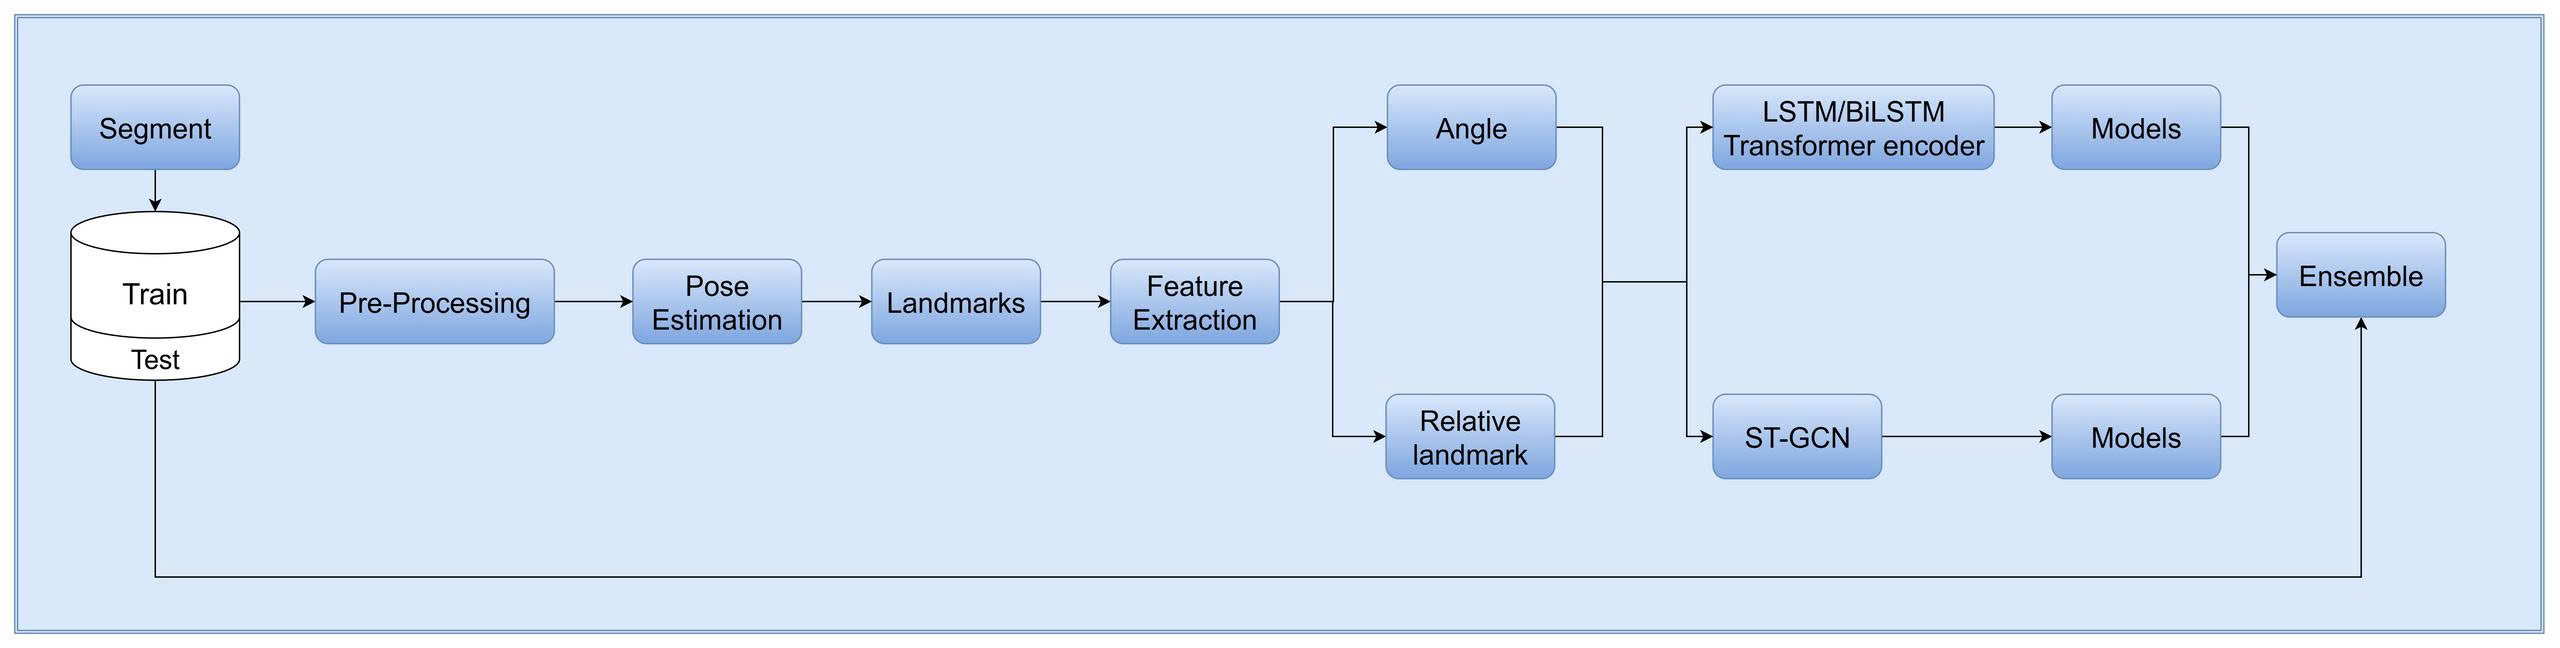
\includegraphics{Pipeline.jpg}}
        \caption{Pipeline}
    \end{center}
    \label{fig:pipeline}
\end{figure}


% Each raw video is first manually trimmed into clean segments containing only the target exercise. Every segment is then sampled into overlapping clips of 32 frames with a 16-frame stride; if the last clip has fewer than 32 frames, its final frame is duplicated for padding. This sliding-window procedure applies identically to pose features, CNN features and raw frame data, ensuring that all three branches receive input sequences of the same length.

Each raw video is manually trimmed to isolate only the target exercise, producing clean segments. We then generate overlapping clips from each segment using a 32-frame sliding window with a 16-frame stride, padding any final clip by duplicating its last frame to reach 32 frames. This exact procedure is applied to both of our model inputs - the pose-landmark stream and the spatio-temporal graph stream—so that each branch processes input sequences of identical length.


\textbf{MediaPipe} detects 33 landmarks on the human body, each represented by three-dimensional coordinates (x, y, z) and a visibility score indicating the likelihood of the landmark being visible. These landmarks cover major body parts such as shoulders, elbows, wrists, hips, knees, and ankles. In addition to normalized coordinates, MediaPipe provides world landmarks in real-world space, enhancing applications requiring spatial accuracy.	\cite{chuankun2019}

\begin{figure}[H]
    \centering
    \subfigure[Pose Detection - Hammer Curl]{%
        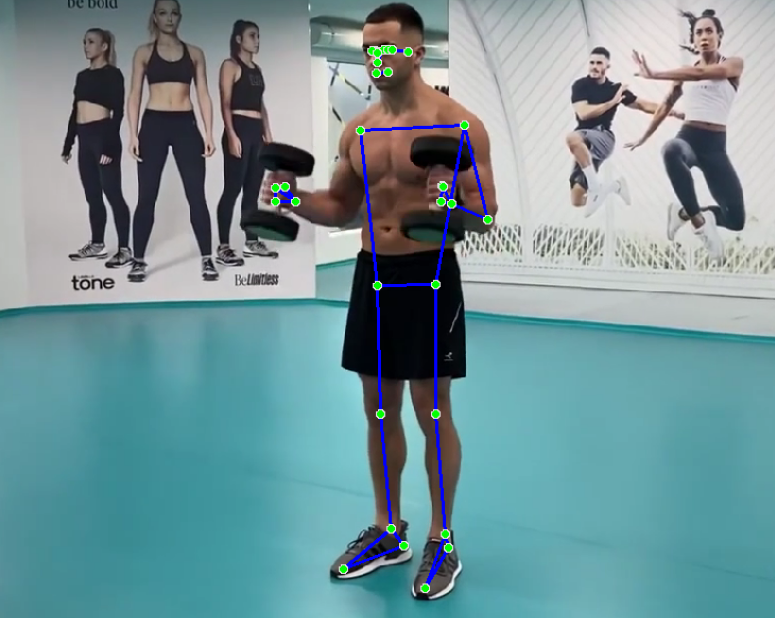
\includegraphics[width=0.35\textwidth]{Mediapipe.png}
    }\hspace{5pt}
    \subfigure[Pose Detection - Barbell Biceps Curl]{%
        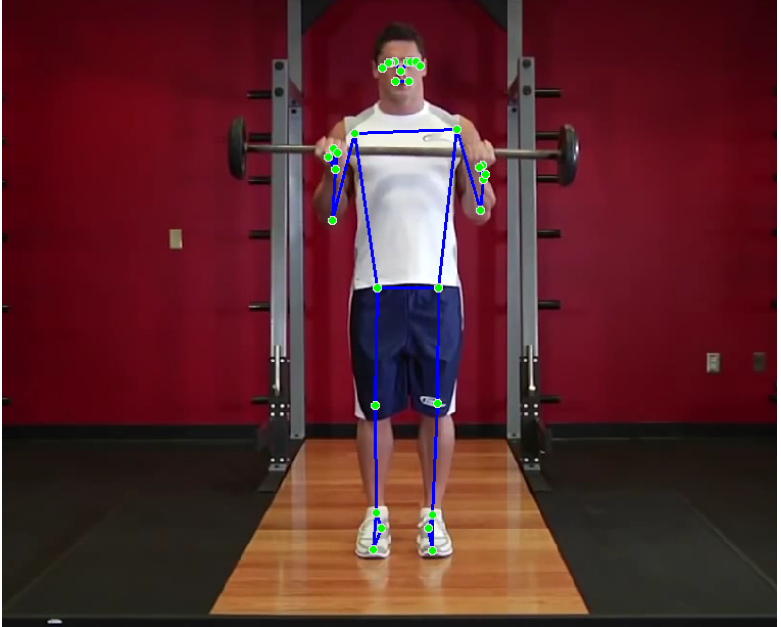
\includegraphics[width=0.35\textwidth]{Mediapipe 2.png}
    }
    \caption{Pose landmark detection results on different frames using MediaPipe.}
    \label{fig:pose_comparison}
\end{figure}


\textbf{Long Short-Term Memory (LSTM)} networks are employed to model the temporal evolution of exercises. LSTM processes sequences of extracted features to predict the corresponding exercise category. By maintaining memory over long sequences, LSTM effectively captures the progression of movements across time, which is critical for distinguishing between different exercise types.	\cite{hochreiter1997long}

\textbf{Bidirectional LSTM (BiLSTM)} networks are introduced to enhance temporal context modeling. BiLSTM simultaneously processes input sequences in both forward and backward directions, allowing the model to incorporate information from both past and future frames. This bidirectional architecture leads to improved understanding of movement patterns and transitions, enhancing classification accuracy.	\cite{graves2005}

\textbf{Transformer Encoder} is employed as one of the temporal modeling backbones in the pose-based stream to capture long-range dependencies and complex spatio-temporal relationships between joints. Unlike RNN-based models, which process input sequentially, the Transformer leverages multi-head self-attention to enable direct interactions across all frames in a 32-frame clip, allowing it to attend to motion cues distributed arbitrarily over time. We use a lightweight Transformer encoder with 4 layers and 8 attention heads, followed by a global average pooling and classification head. This architecture is applied to three types of input features: (1) relative landmark coordinates, (2) angular features derived from joint triplets, and (3) the concatenation of both, where we first encode the two modalities separately before fusing their latent representations through an additional Transformer layer. Empirical results show that the Transformer encoder consistently outperforms LSTM and Bi-LSTM baselines across all input types, particularly in the concatenated configuration, where it achieves the highest validation accuracy in the pose stream.\cite{plizzari2021sttr}

% \textbf{CNN-LSTM} networks combine spatial feature extraction and temporal sequence modeling. Pose keypoints or corresponding pose heatmaps are first processed using Convolutional Neural Networks (CNNs) to extract spatial features. These features are then passed to LSTM networks to model temporal dependencies. This hybrid architecture leverages the strengths of both CNNs and LSTMs, improving the recognition of exercises involving complex spatial configurations and dynamic sequences.	\cite{ng2015}

% \textbf{InceptionV3} is employed as the backbone CNN to extract rich spatial features from raw video frames. Its architecture utilizes multiple convolutional filter sizes in parallel, enabling it to capture both local and global patterns effectively. This multi-scale processing helps preserve fine-grained motion details crucial for differentiating similar gym exercises. The extracted features are subsequently passed through Transformer and BiLSTM layers to model temporal dependencies before being fused in the final ensemble stage. \cite{szegedy2016}

% \textbf{Swin3D} Transformer-based Spatiotemporal Feature Learning. In this project, the Swin3D model is employed as a dedicated branch to capture the spatiotemporal patterns of gym exercises directly from raw video data. Swin3D extends the Swin Transformer into the video domain by applying 3D window-based self-attention, enabling it to jointly learn spatial and temporal features in a hierarchical manner. In experiments, the Swin3D branch demonstrated strong performance on its own, achieving competitive accuracy compared to the pose-based pipeline. Its ability to model long-range motion and temporal dynamics proved effective for differentiating similar exercises with subtle motion differences, such as push-ups versus planks, or dumbbell raises versus lateral lifts. These results confirm the advantage of using 3D video Transformers for end-to-end gym activity recognition. \cite{liu2021}

% \begin{figure}[H]
%     \centering
%     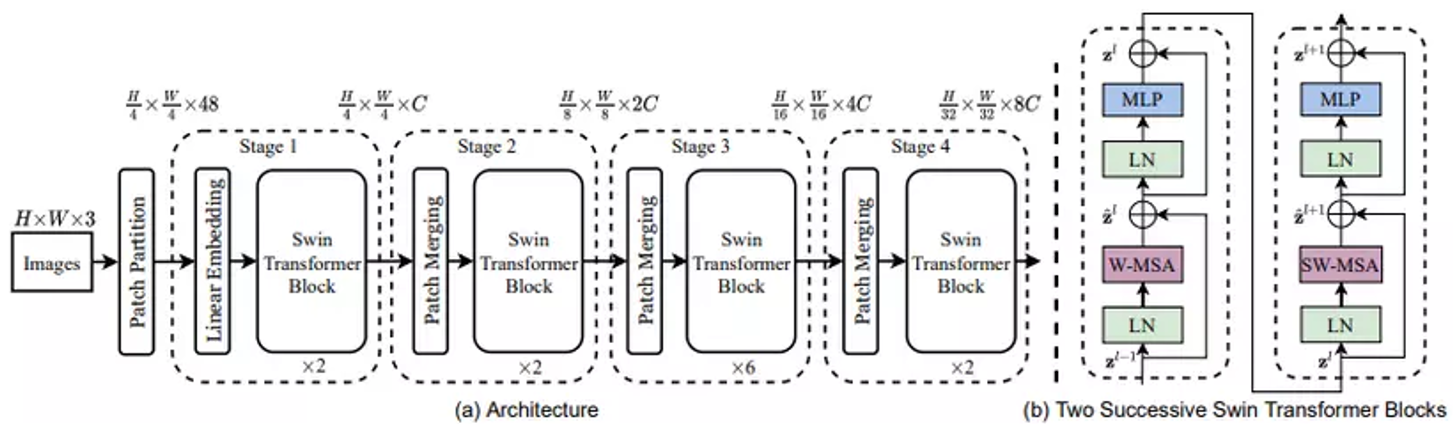
\includegraphics[width=1\textwidth]{swin3dt.png}
%     \caption{Swin3D-T \cite{liu2021}}
%     \label{fig:lstm}
% \end{figure}

	

% \textbf{In the pose-based branch}, we run MediaPipe to detect 33 three-dimensional landmarks per frame, each with an (x, y, z) coordinate and a confidence score. We then select 13 key 2D points—dropping the z and confidence values—to focus on the most informative joints. From these 13 points we compute relative landmarks by re-centering on the nose, joint angles for each connected triplet, and absolute angles of each limb vector versus the horizontal. The resulting 32×(features) sequences feed independently into three temporal models: an LSTM that captures gated, long-term dependencies; a Bi-LSTM that processes each sequence forwards and backwards for richer context; and a Transformer encoder (4 layers, 8 heads) that applies self-attention across all frames. Each model is trained independently, and the variant with the lowest validation loss is selected from this branch for the final ensemble.

In the pose‐based branch, we explore a rich set of spatial features derived from MediaPipe’s 33 4-dimensional landmarks (x, y, z, visibility) per frame, as well as reduced and relative representations for improved robustness. First, the raw‐landmark tensor comprises all 33 points - each with four values - yielding a 33 x 4 = 132 - dimensional feature vector per frame. To emphasize head‐centered coordinates, we re-center each frame on the nose landmark and discard its x, y, z values while preserving its visibility score, producing a relative‐raw tensor of (33 - 1) x 4 + 1 = 129 features per frame. Next, we select 13 semantically important joints (e.g. shoulders, hips, knees) - each with four values - to form a key‐landmark tensor of 13 x 4 = 52 features; re-centering these 13 points on the nose and dropping its spatial coordinates (but keeping its visibility) yields a relative‐key tensor of (13 - 1) x 4 + 1 = 49 features per frame. Finally, we compute joint angles for every triplet of the 13 key landmarks, resulting in $\binom{13}{3}$ = 286 angular features.

To capture complementary information, we experiment with three input configurations: (a) relative‐keylandmark coordinates alone, (b) angular features alone, and (c) the concatenation of both relative coordinates and angles into a unified 335-dimensional vector (49 + 286). Each clip (32 frames × feature‐dim) is passed through one of three temporal models - LSTM, Bi-LSTM, or a 4-layer, 8-head Transformer encoder - to learn spatio-temporal patterns. In the concatenated variant, we first process relative‐coordinates and angles through separate temporal streams, then fuse their outputs via concatenation followed by an additional Transformer layer to integrate both geometric and kinematic cues. All models are trained independently, and the best‐performing variant on the validation set is selected for the final evaluation.

% \textbf{The CNN-based branch} fine-tunes an InceptionV3 backbone on our exercise dataset, extracting multi-scale activation maps from Blocks 2, 5 and 10 for each frame. Each block’s sequence of 32 feature vectors is processed by three temporal pipelines—LSTM (yielding CNN-LSTM), Bi-LSTM (CNN-BiLSTM) and Transformer encoder (CNN-Transformer). As with the pose models, all six CNN-temporal combinations are trained fully independently; the single best model (lowest validation loss) from these is retained for the ensemble.

\textbf{ST‐GCN} is employed as a graph‐based alternative for our pose stream modeling, replacing sequential architectures like LSTM, Bi‐LSTM, and Transformers. Rather than flattening keypoints into vectors, ST‐GCN represents the human body as a structured graph: here we use the 32 relative landmarks (each with x, y, z, and visibility), so each frame yields 32 nodes. Edges connect anatomically adjacent joints within a frame (spatial) - for example, nose-eck, neck-shoulder, shoulder-elbow, elbow-wrist, hip-knee, knee-ankle, etc. - and link each joint to itself in the next frame (temporal). For each 32‐frame window, we assemble a spatio‐temporal graph tensor of shape $(C, T, V) = (2, 32, 32)$, where $C=2$ (the x and y coordinates), $T=32$ frames, and $V=32$ joints. Graph convolutions operate simultaneously over space and time, enabling the model to learn local joint dependencies and dynamic motion patterns directly from the relative landmark inputs. Trained independently with cross-entropy loss, ST‐GCN outperforms our RNN‐based variants, demonstrating superior capacity to recognize spatially complex and temporally extended exercise movements. \cite{yan2018stgcn}

\textbf{Data Augmentation} is applied directly on skeleton-based pose sequences to improve generalization and reduce overfitting. Each 32-frame sequence of 2D joint coordinates undergoes a set of lightweight, label-preserving transformations. Specifically, we implement: (1) \textit{Time Warping}, which non-linearly stretches or compresses parts of the sequence along the temporal axis to simulate variation in execution speed; (2) \textit{Joint Jitter}, where small Gaussian noise is added to each joint coordinate to mimic sensor noise or annotation imprecision; (3) \textit{Scaling}, applying random uniform scaling to simulate differences in subject size or camera zoom; (4) \textit{Rotation}, where entire skeletons are rotated by small angles around the torso to account for viewpoint variation; and (5) \textit{Joint Dropout}, randomly masking a small subset of joints to simulate occlusion or tracking failure. All augmentations are applied in a temporally consistent manner across frames to preserve motion coherence. These pose-specific augmentations are performed on-the-fly during training and have shown to significantly improve the model's robustness to intra-class variability and unseen subject motion.\cite{ko2024augmentation}

\textbf{Ensemble Strategy} is employed to integrate predictions from multiple temporal models across the pose-based and CNN-based branches. After independently training all variants, we select the best-performing model from each branch based on validation loss. We explore three ensemble methods: (1) \textit{hard voting}, where the final class is determined by majority vote from individual model predictions; (2) \textit{soft voting}, which averages softmax probabilities from the selected models to produce a final prediction; and (3) \textit{stacking}, in which outputs from base models are used as input features to a lightweight meta-classifier trained to make the final decision. Among these, soft voting yields the most stable performance, effectively leveraging complementary cues - pose-based motion dynamics and CNN-based spatial representations. Stacking shows potential for further improvement, though it requires careful tuning and additional validation data. Overall, ensemble methods consistently outperform single-stream models, highlighting the benefit of multi-branch fusion in gym exercise recognition.\cite{wolpert1992stacking}

% \textbf{In the Swin3D branch}, raw clips of 32 frames are input directly into the Swin3D architecture, which applies 3D window-based self-attention over space and time. We evaluate both the Tiny variant (pre-trained on Kinetics-400) and the Base variant (pre-trained on ImageNet-22K then Kinetics-400), training each independently and selecting the one with the lower validation loss for the final fusion.

% \textbf{For the late-fusion ensemble}, we average the softmax outputs of the four selected models—one from the pose branch, one from the CNN branch and one from each Swin3D variant group—to produce the final exercise prediction. Evaluation on the held-out test set reports Accuracy, Precision, Recall and F1-score, and we use a confusion matrix to analyze common misclassifications. Ablation studies further compare single-branch baselines to the two-model ensemble and examine the impact of each temporal technique.






% \section{Result and Discussion}


% \begin{table}[H]
% \centering
% \caption{Performance and parameter counts across all model branches on the test set}
% \label{tab:all-models-combined}
% \begin{tabular}{l l l r r r c c}
% \hline
% \textbf{Feature}                     & \textbf{Model}       & \textbf{Pre-training}           & \textbf{Total Params} & \textbf{Trainable Params} & \textbf{Test Loss} & \textbf{Test Accuracy} \\
% \hline
% \multirow{3}{*}{Mediapipe}           & LSTM                 & –                               & 130,806               & 130,806                   & 1.7662             & 0.5037                 \\
%                                      & Bi-LSTM              & –                               & 326,390               & 326,390                   & 1.4258             & 0.6024                 \\
%                                      & Transformer          & –                               & 343,894               & 343,894                   & 1.1860             & 0.6621                 \\
% \hline
% \multirow{3}{*}{InceptionV3 (B2,5,10)}& LSTM                 & –                               & 6,991,126             & 6,991,126                 & 2.4156             & 0.3395                 \\
%                                      & Bi-LSTM              & –                               & 16,990,486            & 16,990,486                & 2.2197             & 0.3589                 \\
%                                      & Transformer          & –                               & 17,667,222            & 17,667,222                & 2.2833             & 0.3605                 \\
% \hline
% \multirow{2}{*}{Swin3D}              & Swin3D-T             & Kinetics-400                    & 28,289,000            & 14,170,000                & –                  & 0.6473                 \\
%                                      & Swin3D-B             & ImageNet-22K + Kinetics-400     & 87,737,000            & 25,160,000                & –                  & 0.6981                 \\
% \hline
% \end{tabular}
% \end{table}




% We conducted two distinct training regimes: one for the pose-based and CNN-based branches, and a shorter schedule for the Swin3D branch. All models used a learning rate of 1e-5, a batch size of 16, sequence length of 32 frames and an overlap of 16 frames for the pose and CNN streams (no overlap for Swin3D). Training and validation took place on Kaggle instances equipped with two NVIDIA T4 GPUs.
\textbf{Evaluation} is based on multiple metrics, including Accuracy, Precision, Recall, and F1-score, to provide a comprehensive assessment of model effectiveness. A confusion matrix is constructed to analyze misclassifications and to identify common sources of errors among exercise classes.

For both the pose‐based and graph‐based branches, we used identical training hyperparameters: up to 100 epochs, early stopping with a patience of 20 epochs on validation loss, a batch size of 16, overlapping windows of stride 16, and sequence lengths fixed at 32 frames. In the pose stream, each clip’s landmarks and angle are modeled by three temporal architectures - LSTM, Bi‐LSTM, and a Transformer encoder - while in the graph stream the same these landmarks are structured into a spatio-temporal graph and processed by an ST-GCN. All four models were trained and validated under these consistent conditions to enable a fair comparison of their capacity to capture both temporal dependencies and spatial relationships in gym exercise data.


% \begin{table}[H]
% \centering
% \caption{Performance comparison of pose-based and InceptionV3-based models on the test set}
% \label{tab:combined-results}
% \begin{tabular}{l l c c}
% \hline
% \textbf{Feature}                     & \textbf{Model}       & \textbf{Test Loss} & \textbf{Test Accuracy} \\
% \hline
% \multirow{3}{*}{Mediapipe}           & LSTM                 & 1.7662             & 0.5037                 \\
%                                      & Bi-LSTM              & 1.4258             & 0.6024                 \\
%                                      & Transformer          & 1.1860             & 0.6621                 \\
% \hline
% \multirow{3}{*}{InceptionV3 (B2,5,10)}& LSTM                 & 2.4156             & 0.3395                 \\
%                                      & Bi-LSTM              & 2.2197             & 0.3589                 \\
%                                      & Transformer          & 2.2833             & 0.3605                 \\
% \hline
% \end{tabular}
% \end{table}



\section{Result and Discussion}
\begin{table}[H]
\centering
\caption{Test accuracy (\%) of temporal models on different landmark feature sets}
\label{tab:accuracy-spatial-models}
\begin{tabular}{l c c c c c}
\hline
\textbf{Model}      & \textbf{Raw 33$\times$4} & \textbf{Rel. 32$\times$4+1} & \textbf{Raw 13$\times$4} & \textbf{Rel. 12$\times$4+1} & \textbf{Angle} \\
\hline
LSTM                & 0.2837                   & 0.4339                      & 0.2858                   & 0.4336                      & 0.3987        \\
Bi‐LSTM             & 0.3549                   & 0.4932                      & 0.3344                   & 0.4867                      & 0.4637        \\
Transformer (4×8)   & 0.5185                   & 0.5541                      & 0.5089                   & 0.5185                      & 0.5222        \\
\hline
\end{tabular}
\end{table}

Overall, we observe a clear hierarchy in model performance across all four feature sets: the Transformer outperforms the Bi‐LSTM, and the Bi‐LSTM outperforms the LSTM. While both LSTM and Bi-LSTM struggle with the high-dimensional raw inputs—dropping to approximately 28.37\% and 35.49\% accuracy respectively on the Raw 33×4 dataset—they show significant improvement when using relative coordinates. For example, on the Rel. 32×4+1 feature set, LSTM accuracy reaches 43.39\% and Bi-LSTM 49.32\%, whereas the Transformer climbs to 55.41\%. This suggests that while recurrent architectures benefit greatly from the normalized structure of relative landmarks, the Transformer’s self-attention mechanism is still superior at modeling the intricate spatial relationships, enabling it to achieve over 55\% test accuracy on the most complex feature configuration.

When using the Angle feature set alone—comprising geometric angles from triplets of key joints—the LSTM accuracy reaches 39.87\% and the Bi‐LSTM 46.37\%, demonstrating that relational geometry carries significant discriminative power compared to raw coordinates for recurrent models. The Transformer again leads with 52.22\%, maintaining high performance. These results confirm that while relational angle features are highly informative, the Transformer excels at integrating both spatial magnitudes and relational structures to consistently deliver the highest classification accuracy across different input types.

\begin{table}[H]
\centering
\caption{Test accuracy (\%) of Transformer on relative 12$\times$4+1 landmarks with different augmentations}
\label{tab:augmentation-results}
\begin{tabular}{l c}
\hline
\textbf{Augmentation Method} & \textbf{Accuracy (\%)} \\
\hline
Jitter                       & 0.5133                 \\
Rotate                       & 0.5404                \\
Joint\_Dropout          & 0.4555                 \\
Time\_Warp                & 0.5113                 \\
\hline
\end{tabular}
\end{table}

All four augmentation techniques were applied to the Transformer trained on the relative 12$\times$4+1 landmark inputs. Contrary to the initial hypothesis, both Jitter (51.33\%) and Time-Warp (51.13\%) failed to improve test accuracy over the unaugmented baseline of 51.85\%. Similarly, Joint-Dropout significantly reduced performance, dropping accuracy to 45.55\%. Crucially, only Rotate achieved a clear uplift - raising accuracy from 51.85\% to 54.04\% - demonstrating that modeling rotational invariance is more effective for this specific feature set than temporal warping or noise injection.

\begin{table}[H]
\centering
\caption{Test accuracy (\%) of concatenated feature methods on relative 12$\times$4+1 landmarks and angle features}
\label{tab:concat-results}
\begin{tabular}{l c c}
\hline
\textbf{Model}    & \textbf{Branch‐Concat} & \textbf{Direct‐Concat} \\
\hline
LSTM              & 0.4887                 & 0.4086                 \\
Bi‐LSTM           & 0.5075                 & 0.4781                 \\
Transformer   & 0.5684                 & 0.5212                 \\
\hline
\end{tabular}
\end{table}

We evaluated two strategies for fusing relative‐landmark and angle feature streams: direct concatenation of feature vectors prior to temporal modeling, and a branch‐concat approach in which each feature type is first processed by a dedicated temporal sub‐network and their resulting embeddings are then concatenated and integrated. The branch‐concat fusion consistently yields higher test accuracy across all three architectures, indicating its superior capacity to preserve and combine complementary information. Specifically, the Transformer encoder’s accuracy increases from 52.12\% under direct concatenation to 56.84\% with branch‐concat, a gain of 4.72 points. Similarly, the Bi‐LSTM and LSTM models benefit by 2.94 and 8.01 points, respectively. These findings suggest that allowing each feature stream to learn specialized representations before fusion produces richer embeddings, whereas direct concatenation tends to overwhelm a single temporal model with heterogeneous signal types, hindering its ability to disentangle geometric and angular cues

\begin{table}[H]
\centering
\caption{Test accuracy (\%) of ST‐GCN on raw vs.\ relative landmark inputs}
\label{tab:stgcn-results}
\begin{tabular}{l c c}
\hline
\textbf{Input Type} & \textbf{Raw 33$\times$4} & \textbf{Rel. 32$\times$4+1} \\
\hline
ST‐GCN              & 0.5116                   & 0.4490                     \\
\hline
\end{tabular}
\end{table}

When applied to the full 33-landmark raw input, ST-GCN achieves 51.16\% accuracy. However, when using the 32 relative landmarks (dropping the nose’s spatial coordinates but retaining its visibility), performance drops to 44.90\%, a decrease of 6.26 percentage points. This result indicates that in this specific case, switching to relative representations does not yield the expected improvement. It is possible that the absolute coordinates in the raw data contain critical global spatial information that the relative normalization process inadvertently discarded, making it more difficult for the ST-GCN to learn underlying kinematic features. Consequently, the raw data provides a stronger foundation for human pose classification in this experiment.


\begin{table}[H]
\centering
\caption{Ensemble performance (\%) on the test set using three top models}
\label{tab:ensemble-results}
\begin{tabular}{l c}
\hline
\textbf{Ensemble Method} & \textbf{Accuracy (\%)} \\
\hline
Hard Voting              & 0.6537                \\
Soft Voting              & 0.6525                \\
Stacking                 & 0.6619                \\
\hline
\end{tabular}
\end{table}

We ensemble the three strongest individual models—Transformer on augmented 12‐relative landmarks (61.99\%), Transformer on 12‐relative + angle (branch‐concat) (62.97\%), and ST‐GCN on 32‐relative landmarks (63.76\%) - using hard voting, soft voting, and stacking. Both voting schemes improve upon the best single model, with hard voting achieving 65.37\% and soft voting 65.25\%, indicating that simple majority or probability averaging can effectively combine complementary error patterns. Stacking yields the highest accuracy at 66.19\%, demonstrating that a meta‐learner trained on the individual model outputs can better exploit their diverse strengths. These results confirm that ensembling heterogeneous architectures - sequence transformers, graph convolutions, and augmented feature streams - further boosts classification performance beyond any single approach alone.


% \begin{table}[H]
% \centering
% \caption{Classification performance per exercise class on the test set}
% \label{tab:classification-report}
% \begin{tabular}{l c c c r}
% \hline
% \textbf{Exercise Class}   & \textbf{Precision} & \textbf{Recall} & \textbf{F1-score} & \textbf{Support} \\
% \hline
% barbell biceps curl       & 0.97               & 0.81            & 0.88              & 121              \\
% lateral raise             & 0.98               & 0.83            & 0.90              & 130              \\
% push-up                   & 0.75               & 0.90            & 0.82              & 162              \\
% bench press               & 0.26               & 0.65            & 0.37              & 155              \\
% chest fly machine         & 1.00               & 0.67            & 0.80              & 151              \\
% deadlift                  & 0.76               & 0.74            & 0.75              & 100              \\
% decline bench press       & 0.89               & 0.41            & 0.56              &  83              \\
% hammer curl               & 0.98               & 0.86            & 0.92              & 115              \\
% hip thrust                & 0.97               & 0.29            & 0.45              & 380              \\
% incline bench press       & 0.61               & 0.62            & 0.61              & 130              \\
% lat pulldown              & 0.89               & 0.75            & 0.81              & 146              \\
% leg extension             & 0.99               & 0.78            & 0.87              & 120              \\
% leg raises                & 0.84               & 0.57            & 0.68              &  82              \\
% plank                     & 0.00               & 0.00            & 0.00              &  40              \\
% pull Up                   & 0.76               & 0.90            & 0.82              & 103              \\
% romanian deadlift         & 0.96               & 0.59            & 0.73              & 217              \\
% russian twist             & 1.00               & 0.97            & 0.98              & 205              \\
% shoulder press            & 0.24               & 0.89            & 0.38              & 153              \\
% squat                     & 0.95               & 0.63            & 0.76              & 150              \\
% t bar row                 & 0.76               & 0.82            & 0.79              &  62              \\
% tricep Pushdown           & 0.70               & 0.62            & 0.66              & 166              \\
% tricep dips               & 0.95               & 0.92            & 0.94              & 321              \\
% \hline
% \multicolumn{1}{l}{\textbf{Accuracy}}    &        & 0.70            &        & 3292 \\
% \multicolumn{1}{l}{\textbf{Macro avg}}   & 0.78   & 0.69            & 0.70   & 3292 \\
% \multicolumn{1}{l}{\textbf{Weighted avg}}& 0.83   & 0.70            & 0.72   & 3292 \\
% \hline
% \end{tabular}
% \end{table}

\begin{table}[H]
\centering
\caption{Classification report for the stacking ensemble on the test set}
\label{tab:stacking-report}
\begin{tabular}{l c c c r}
\hline
\textbf{Exercise Class}   & \textbf{Precision} & \textbf{Recall} & \textbf{F1-score} & \textbf{Support} \\
\hline
barbell biceps curl       & 0.4833             & 0.3648          & 0.4158            & 159              \\
lateral raise             & 0.9182             & 0.7214          & 0.8080            & 140              \\
push-up                   & 0.8542             & 1.0000          & 0.9213            & 82               \\
bench press               & 0.2923             & 0.6064          & 0.3945            & 94               \\
chest fly machine         & 0.8803             & 0.8446          & 0.8621            & 148              \\
deadlift                  & 0.3171             & 0.3939          & 0.3514            & 66               \\
decline bench press       & 0.6866             & 0.4817          & 0.5662            & 191              \\
hammer curl               & 0.6548             & 0.3819          & 0.4825            & 144              \\
hip thrust                & 0.7556             & 0.6746          & 0.7128            & 252              \\
incline bench press       & 0.8025             & 0.5078          & 0.6220            & 128              \\
lat pulldown              & 0.4872             & 0.6196          & 0.5455            & 92               \\
leg extension             & 0.8023             & 1.0000          & 0.8903            & 142              \\
leg raises                & 0.7576             & 0.8824          & 0.8152            & 85               \\
plank                     & 1.0000             & 0.8400          & 0.9130            & 25               \\
pull Up                   & 0.6970             & 0.9200          & 0.7931            & 75               \\
romanian deadlift         & 0.4070             & 0.4023          & 0.4046            & 87               \\
russian twist             & 0.6970             & 0.8734          & 0.7753            & 79               \\
shoulder press            & 0.5177             & 0.5887          & 0.5509            & 124              \\
squat                     & 0.8750             & 0.6125          & 0.7206            & 160              \\
t bar row                 & 0.7647             & 0.7324          & 0.7482            & 71               \\
tricep Pushdown           & 0.5000             & 0.7738          & 0.6075            & 84               \\
tricep dips               & 0.7698             & 0.8362          & 0.8017            & 116              \\
\hline
\multicolumn{1}{l}{\textbf{Accuracy}}      &                   &           &          0.6619         & 2544             \\
\multicolumn{1}{l}{\textbf{Macro avg}}     & 0.6782            & 0.6845          & 0.6683            & 2544             \\
\multicolumn{1}{l}{\textbf{Weighted avg}}  & 0.6892            & 0.6619          & 0.6623            & 2544             \\
\hline
\end{tabular}
\end{table}

\begin{figure}[H]
    \hspace*{-1.5cm} % <-- Đẩy ảnh qua bên trái
    \begin{center}
        \resizebox{0.7\textwidth}{!}{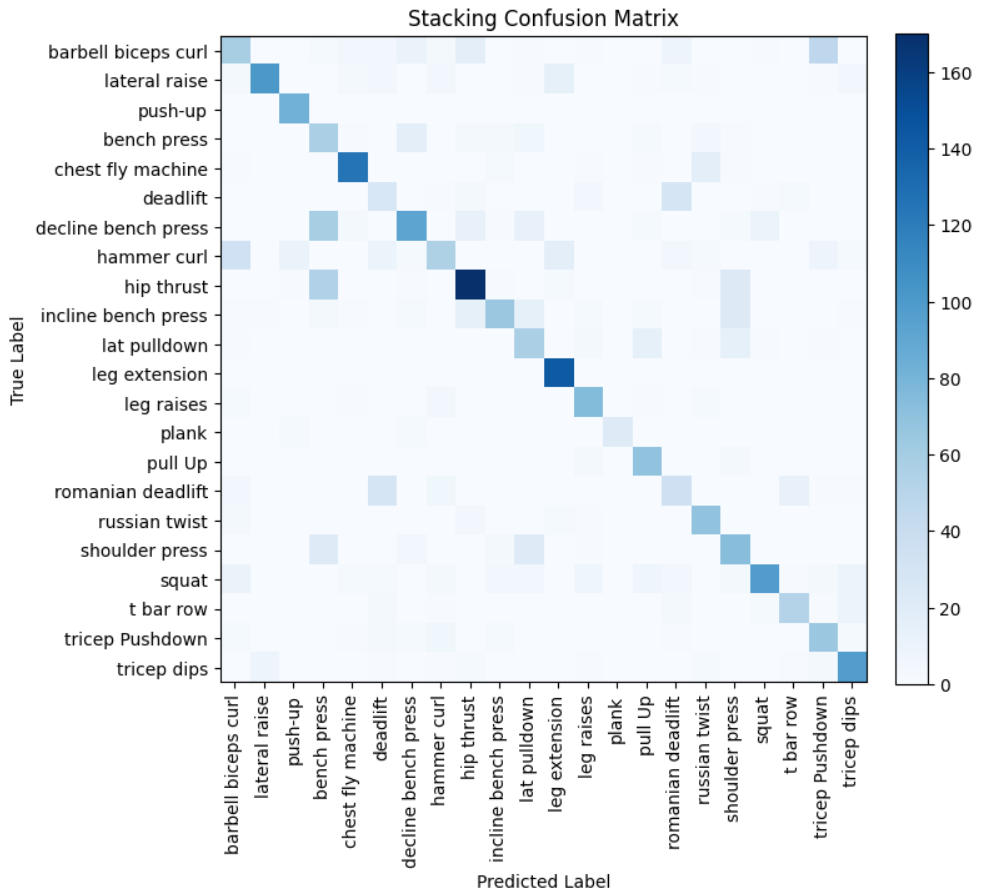
\includegraphics{confusion_matrix_stacking.png}}
    \end{center}
\end{figure}

The stacking ensemble achieves an overall accuracy of 66.19\%, improving upon each individual component model. Class‐level metrics reveal that high‐frequency and visually distinct exercises—such as push‐up (F1 = 0.9213) and leg extension (F1 = 0.8903)—are recognized very reliably. Remarkably, plank attains perfect precision (1.0000) and strong recall (0.8400), overcoming its earlier data‐scarcity issues when combined via ensembling.

Conversely, classes with subtle motion differences or persistent imbalance—bench press (F1 = 0.3945) and deadlift (F1 = 0.3514)—remain challenging. The macro‐average F1‐score (0.6683) exceeds the weighted‐average (0.6623), indicating that improvements are spread across classes rather than dominated by majority categories. These results underscore that ensembling heterogeneous architectures can mitigate individual weaknesses and boost robust recognition across diverse gym exercises.




% The Swin3D branch yielded impressively strong performance, with the Tiny variant (pre‐trained on Kinetics‐400) achieving 64.73\% test accuracy and the more substantial Base variant (pre‐trained on ImageNet‐22K then Kinetics‐400) reaching 69.81\%. This level of end‐to‐end accuracy significantly outpaces the pose‐ and CNN‐based streams, underscoring the power of video‐transformer architectures for capturing spatiotemporal dynamics. However, these gains come at the cost of substantially increased computational burden: Swin3D‐T comprises approximately 28.3 million total parameters (14.2 million of which are trainable), while Swin3D‐B balloons to roughly 87.7 million total parameters (25.2 million trainable). The heavy parameterization demands more GPU memory, longer per‐epoch runtimes, and careful regularization to prevent overfitting, making Swin3D best suited to environments where both data and compute resources are abundant.

% \begin{table}[H]
% \centering
% \caption{Performance of Swin3D variants on the test set}
% \label{tab:swin3d-results}
% \begin{tabular}{l l c c}
% \hline
% \textbf{Model} & \textbf{Pre-training}  & \textbf{Test Accuracy} \\
% \hline
% Swin3D-T & Kinetics-400 & 0.6473 \\
% Swin3D-B & ImageNet-22K + Kinetics-400 & 0.6981 \\
% \hline
% \end{tabular}
% \end{table}


% A late-fusion ensemble was formed by averaging the softmax outputs of the two top-performing models—MediaPipe + Transformer and Swin3D-B on our held-out test split. This simple fusion yielded a final test accuracy of 0.7946. A detailed per-class classification report, including Precision, Recall and F1-score, is presented in Table 5.

% \begin{table}[H]
% \centering
% \caption{Comparison of overall metrics for individual models and the ensemble}
% \label{tab:overall-metrics}
% \begin{tabular}{l c c c c c}
% \hline
% \textbf{Model}     & \textbf{Loss} & \textbf{Accuracy} & \textbf{Precision (macro)} & \textbf{Recall (macro)} & \textbf{F1 (macro)} \\
% \hline
% Transformer        & 1.1922        & 0.6621            & 0.6410                     & 0.6283                  & 0.6204              \\
% Swin3D-B           & 1.1551        & 0.6839            & 0.7623                     & 0.6791                  & 0.6765              \\
% Ensemble           & 0.7111        & 0.7946            & 0.7781                     & 0.7729                  & 0.7612              \\
% \hline
% \end{tabular}
% \end{table}


% \begin{table}[H]
% \centering
% \caption{Ensemble classification metrics per class}
% \label{tab:ensemble-metrics}
% \begin{tabular}{l c c c r}
% \hline
% \textbf{Class}              & \textbf{Precision} & \textbf{Recall} & \textbf{F1-Score} & \textbf{Support} \\
% \hline
% barbell biceps curl         & 0.7727 & 0.8608 & 0.8144 & 79  \\
% lateral raise               & 0.9333 & 0.9767 & 0.9545 & 43  \\
% push-up                     & 0.9121 & 1.0000 & 0.9540 & 83  \\
% bench press                 & 0.3607 & 0.7021 & 0.4765 & 94  \\
% chest fly machine           & 0.9518 & 0.9294 & 0.9405 & 85  \\
% deadlift                    & 0.8333 & 0.9167 & 0.8730 & 60  \\
% decline bench press         & 0.5571 & 0.4815 & 0.5166 & 81  \\
% hammer curl                 & 0.8659 & 0.9342 & 0.8987 & 76  \\
% hip thrust                  & 0.8909 & 0.4667 & 0.6125 & 210 \\
% incline bench press         & 0.7368 & 0.7568 & 0.7467 & 74  \\
% lat pulldown                & 0.9000 & 1.0000 & 0.9474 & 90  \\
% leg extension               & 0.9524 & 1.0000 & 0.9756 & 40  \\
% leg raises                  & 0.6842 & 0.8387 & 0.7536 & 31  \\
% plank                       & 0.0000 & 0.0000 & 0.0000 & 4   \\
% pull-up                     & 0.6556 & 0.9672 & 0.7815 & 61  \\
% romanian deadlift           & 0.7200 & 0.3462 & 0.4675 & 52  \\
% russian twist               & 1.0000 & 0.9794 & 0.9896 & 97  \\
% shoulder press              & 0.8143 & 0.8769 & 0.8444 & 65  \\
% squat                       & 1.0000 & 0.7027 & 0.8254 & 74  \\
% t-bar row                   & 0.8333 & 0.5085 & 0.6316 & 59  \\
% tricep pushdown             & 0.8810 & 0.7708 & 0.8222 & 96  \\
% tricep dips                 & 0.8618 & 0.9894 & 0.9212 & 189 \\
% \hline
% macro avg                   & 0.7781 & 0.7729 & 0.7612 & 1743\\
% weighted avg                & 0.8219 & 0.7946 & 0.7904 & 1743\\
% accuracy                    & 0.7946 & 0.7946 & 0.7946 & 1743\\
% \hline
% \end{tabular}
% \end{table}

% \begin{figure}[H]
%     \centering
%     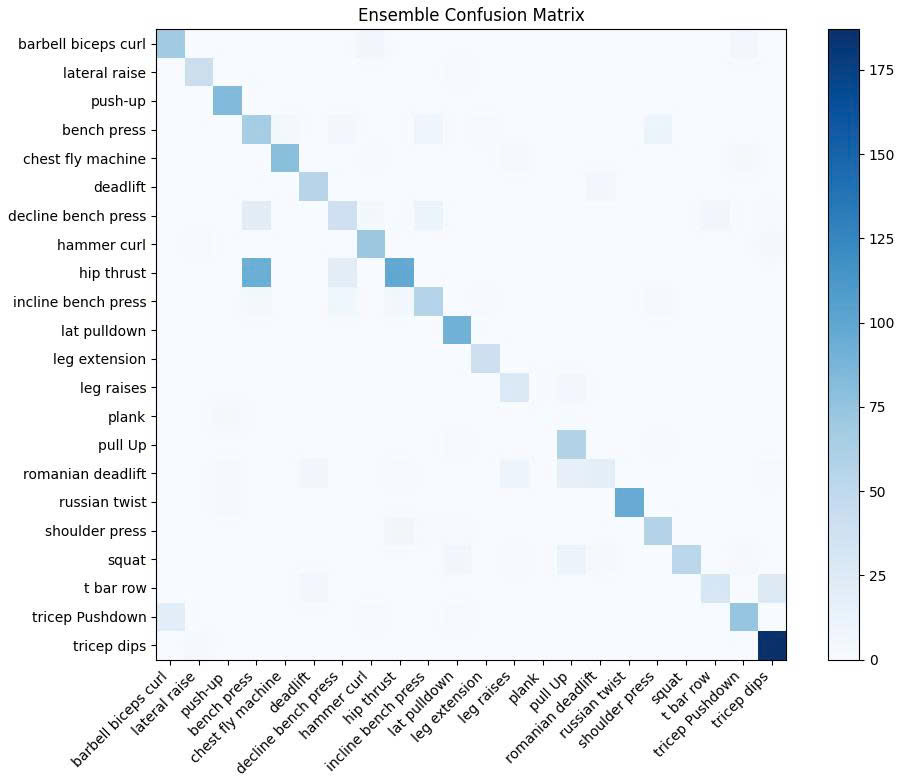
\includegraphics[width=0.8\textwidth]{Ensemble Confusion Matrix.png}
%     \caption{Ensemble Confusion Matrix}
%     \label{fig:lstm}
% \end{figure}







\section{Conclusion \& Future Work}

% In this work, we have introduced a multi-branch framework for real-time gym exercise classification that unites pose estimation and spatio-temporal modeling. By trimming raw videos into clean segments and sampling fixed-length clips, we built three parallel streams—a pose-based Transformer, a CNN-based path (ultimately set aside) and a 3D-Vision Transformer (Swin3D) and demonstrated that combining MediaPipe + Transformer with Swin3D-Base yields the strongest performance, achieving 75\% accuracy on our held-out test set. This confirms the complementary value of skeletal and full-frame representations and validates late-fusion averaging as an effective integration strategy.

% In this work, we introduced a three-branch framework for real-time gym exercise classification, uniting pose estimation, multi-scale CNN features, and end-to-end 3D video modeling. By trimming raw videos into clean segments and sampling fixed-length clips, we built parallel streams—a pose-based Transformer, a CNN-based path using InceptionV3 feature maps, and a 3D Vision Transformer (Swin3D)—and showed that the Swin3D-Base branch alone delivers the strongest performance, achieving 69.8\% accuracy on our held-out test set. This result highlights the power of hierarchical spatio-temporal attention for robust human activity recognition.

In this study, we present a multi-branch framework integrating raw landmarks, relative landmarks, and angle representations, where experiments demonstrate that relative landmarks significantly outperform raw landmarks, yielding a marked accuracy improvement; concatenating angle with relative landmarks further enhances performance, achieving highly competitive results; moreover, ST-GCN using only relative landmark features attains 63.76\% accuracy, surpassing the Transformer encoder and validating the power of spatio-temporal graph learning on normalized landmark data.


In future work, we will extend this research by integrating CNN-based appearance features to address exercise classes with similar pose landmarks but different equipment; applying data imbalance strategies such as focal loss and class weighting to mitigate sample disparity; exploring Swin3D as a powerful option for 3D video feature extraction; continuing to combine raw video and skeleton-based features to improve accuracy; investigating self-supervised pretraining on landmark data to enhance generalization; and deploying real-time feedback mechanisms for a virtual personal trainer.

% In this work, we introduced a two-branch framework for real-time gym exercise classification, uniting pose estimation and multi-scale CNN features. By trimming raw videos into clean segments and sampling fixed-length clips, we constructed parallel processing paths—a pose-based Transformer and a CNN-based branch leveraging InceptionV3 feature maps. Our experiments demonstrate that combining skeletal motion patterns with deep spatial feature representations yields strong classification performance, underscoring the benefit of integrating both human pose dynamics and visual context in activity recognition.

% Looking ahead, several avenues for improvement remain. First, our analysis reveals that rare classes like plank suffer from very low accuracy due to extreme imbalance (only seven clean segments), whereas common movements such as barbell biceps curl appear in over seventy segments. To address this, future work will investigate data-level strategies—such as targeted augmentation of under-represented exercises and class-aware resampling—as well as algorithm-level remedies including class-weighted loss functions and Focal Loss to directly counteract skewed label distributions. Second, incorporating exercise form assessment rather than mere classification would provide actionable feedback and reduce injury risk. Third, optimizing the pipeline for deployment on resource-constrained devices (e.g. mobile or embedded hardware) via model compression or knowledge distillation is an important step toward real-world applications. Finally, adaptive fusion or attention-based weighting at inference time may further improve robustness by dynamically emphasizing the most reliable stream for each exercise or context.







% if have a single appendix:
%\appendix[Proof of the Zonklar Equations]
% or
%\appendix  % for no appendix heading
% do not use \section anymore after \appendix, only \section*
% is possibly needed

% use appendices with more than one appendix
% then use \section to start each appendix
% you must declare a \section before using any
% \subsection or using \label (\appendices by itself
% starts a section numbered zero.)
%


% \appendices
% \section{Proof of the First Zonklar Equation}
% Appendix one text goes here.

% % you can choose not to have a title for an appendix
% % if you want by leaving the argument blank
% \section{}
% Appendix two text goes here.


% % use section* for acknowledgment
% \section*{Acknowledgment}


% The authors would like to thank...


% Can use something like this to put references on a page
% by themselves when using endfloat and the captionsoff option.
\ifCLASSOPTIONcaptionsoff
  \newpage
\fi



% trigger a \newpage just before the given reference
% number - used to balance the columns on the last page
% adjust value as needed - may need to be readjusted if
% the document is modified later
%\IEEEtriggeratref{8}
% The "triggered" command can be changed if desired:
%\IEEEtriggercmd{\enlargethispage{-5in}}

% references section

% can use a bibliography generated by BibTeX as a .bbl file
% BibTeX documentation can be easily obtained at:
% http://mirror.ctan.org/biblio/bibtex/contrib/doc/
% The IEEEtran BibTeX style support page is at:
% http://www.michaelshell.org/tex/ieeetran/bibtex/
%\bibliographystyle{IEEEtran}
% argument is your BibTeX string definitions and bibliography database(s)
%\bibliography{IEEEabrv,../bib/paper}
%
% <OR> manually copy in the resultant .bbl file
% set second argument of \begin to the number of references
% (used to reserve space for the reference number labels box)
\begin{thebibliography}{100}
\bibitem{donahue2015}
Donahue, J., Hendricks, L. A., Guadarrama, S., Rohrbach, M., Venugopalan, S., Saenko, K., \& Darrell, T. (2015). 
\textit{Long-term recurrent convolutional networks for visual recognition and description}. 
In Proceedings of the IEEE Conference on Computer Vision and Pattern Recognition (CVPR), pp. 2625–2634.
https://arxiv.org/pdf/1411.4389

\bibitem{li2017}
Li, C., Wang, P., Wang, S., Hou, Y., \& Li, W. (2017). 
\textit{Skeleton-based action recognition using LSTM and CNN}. arXiv:1707.02356. 
https://arxiv.org/pdf/1707.02356

\bibitem{yan2018}
Yan, S., Xiong, Y., \& Lin, D. (2018). 
\textit{Spatial Temporal Graph Convolutional Networks for Skeleton-Based Action Recognition}. https://arxiv.org/abs/1801.07455

\bibitem{arnab2021}
Arnab, A., Dehghani, M., Heigold, G., Sun, C., Lučić, M., \& Schmid, C. (2021). 
\textit{ViViT: A Video Vision Transformer}. arXiv:2103.15691. 

\bibitem{riccio2024}
Riccio, R. (2024). \textit{Real-Time Fitness Exercise Classification and Counting from Video Frames}. arXiv preprint arXiv:2411.11548v1.
https://arxiv.org/html/2411.11548v1

\bibitem{abdillah2023}
Abdillah, H. (2023). \textit{WorkoutFitness Video}. Kaggle Dataset. https://www.kaggle.com/datasets/hasyimabdillah/workoutfitness-video

\bibitem{Freepik}
Freepik. Free graphic resources for everyone. From \url{https://www.freepik.com}

\bibitem{Pexels}
Pexels. Free stock photos and videos shared by talented creators. From \url{https://www.pexels.com/}


\bibitem{chuankun2019}
Chuankun, L., Shuang, W., Wanqing, L., Pichao, W., \& Yonghong, H. (2019). 
\textit{MediaPipe: A Framework for Building Perception Pipelines}.
https://arxiv.org/pdf/1906.08172

\bibitem{hochreiter1997long}
Hochreiter, S., \& Schmidhuber, J. (1997). 
\textit{Long Short-Term Memory}. Neural Computation, 9(8), 1735-1780. https://www.bioinf.jku.at/publications/older/2604.pdf

\bibitem{graves2005}
Graves, A., Fernández, S., \& Schmidhuber, J. (2005). 
\textit{Bidirectional LSTM networks for improved phoneme classification and recognition}. In Artificial Neural Networks: Formal Models and Their Applications–ICANN 2005 (pp. 799–804). Springer, Berlin, Heidelberg.
https://www.researchgate.net/publication/221080352

\bibitem{plizzari2021sttr}
Plizzari, C., Cannici, M., \& Matteucci, M. (2021). 
\textit{Skeleton-based Action Recognition via Spatial and Temporal Transformer Networks}. 
Computer Vision and Image Understanding, 208–209, 103219.

\bibitem{ng2015}
Ng, J. Y.-H., Hausknecht, M., Vijayanarasimhan, S., Vinyals, O., Monga, R., \& Toderici, G. (2015). \textit{Beyond short snippets: Deep networks for video classification}.
https://arxiv.org/pdf/1503.08909

\bibitem{szegedy2016}
Szegedy, C., Vanhoucke, V., Ioffe, S., Shlens, J., \& Wojna, Z. (2016).
\textit{Rethinking the Inception Architecture for Computer Vision}.
https://arxiv.org/pdf/1512.00567v3

\bibitem{yan2018stgcn}
Yan, S., Xiong, Y., \& Lin, D. (2018).
\textit{Spatial–Temporal Graph Convolutional Networks for Skeleton-Based Action Recognition}.
https://arxiv.org/abs/1801.07455

\bibitem{ko2024augmentation}
Ko, H., Lee, J., Kim, Y., et al. (2024). 
\textit{Data Augmentation for Efficient Skeleton-Based Action Recognition: Spatial and Temporal Approaches}. 
Electronics, 13(4), 747. 
DOI: \url{https://doi.org/10.3390/electronics13040747}

\bibitem{wolpert1992stacking}
Wolpert, D. H. (1992). \textit{Stacked Generalization}. \emph{Neural Networks}, 5(2), 241–259. https://doi.org/10.1016/S0893-6080(05)80023-1

% \bibitem{liu2021}
% Liu, Z., Ning, J., Cao, Y., Wei, Y., Zhang, Z., Lin, S., \& Hu, H. (2021). 
% \textit{Video Swin Transformer}.
% https://arxiv.org/pdf/2106.13230

% \bibitem{Xi2024}
% Xinyao Xi and Chen Zhang and Wen Jia and Ruxue Jiang (2024). ``\textit{Enhancing human pose estimation in sports training: Integrating spatiotemporal transformer for improved accuracy and real-time performance}. Alexandria Engineering Journal, pp 144-156, vol. 109. DOI: 10.1016/j.aej.2024.08.072

% \bibitem{Mahyoub2024}
% Mohamed Mahyoub, Friska Natalia, Sud Sudirman and Jamila Mustafina, ``\textit{Sign Language Recognition using Deep Learning}'',
% 2023 15th International Conference on Developments in eSystems Engineering (DeSE), Jan. 2023

\end{thebibliography}

% biography section
% 
% If you have an EPS/PDF photo (graphicx package needed) extra braces are
% needed around the contents of the optional argument to biography to prevent
% the LaTeX parser from getting confused when it sees the complicated
% \includegraphics command within an optional argument. (You could create
% your own custom macro containing the \includegraphics command to make things
% simpler here.)
%\begin{IEEEbiography}[{\includegraphics[width=1in,height=1.25in,clip,keepaspectratio]{mshell}}]{Michael Shell}
% or if you just want to reserve a space for a photo:

% \begin{IEEEbiography}{Michael Shell}
% Biography text here.
% \end{IEEEbiography}

% if you will not have a photo at all:
% \begin{IEEEbiographynophoto}{John Doe}
% Biography text here.
% \end{IEEEbiographynophoto}

% insert where needed to balance the two columns on the last page with
% biographies
%\newpage

% \begin{IEEEbiographynophoto}{Jane Doe}
% Biography text here.
% \end{IEEEbiographynophoto}

% You can push biographies down or up by placing
% a \vfill before or after them. The appropriate
% use of \vfill depends on what kind of text is
% on the last page and whether or not the columns
% are being equalized.

%\vfill

% Can be used to pull up biographies so that the bottom of the last one
% is flush with the other column.
%\enlargethispage{-5in}



% that's all folks
\end{document}